\documentclass{article}

\newcommand{\version}{@LIBSUPERMESH_VERSION@}


\usepackage{amsmath}
\usepackage{amssymb}
\usepackage{enumitem}
\usepackage[a4paper,left=20mm,right=20mm]{geometry}
\usepackage{graphicx}
\usepackage[pdfborder={0 0 0}]{hyperref}
\usepackage{listings}
\usepackage{natbib}
\usepackage{textcomp}

\renewcommand{\ttdefault}{pcr}

\begin{document}

\title{libsupermesh version \version}
\date{April 2016}
\author{James R. Maddison \\ School of Mathematics and Maxwell Institute for Mathematical Sciences, \\ University of Edinburgh, UK\footnote{E-mail: \href{mailto:j.r.maddison@ed.ac.uk}{j.r.maddison@ed.ac.uk}} \\
   \and Iakovos Panourgias \\ EPCC, University of Edinburgh, UK, \\
   \and Patrick E. Farrell \\ Mathematical Institute, University of Oxford, UK, \\ Center for Biomedical Computing, Simula Research Laboratory, Oslo, Norway}

\maketitle

\tableofcontents

\section{Introduction}

libsupermesh is a Fortran 2008 library for serial and parallel mesh
intersection, or supermeshing \citep{farrell2009,farrell2009a}. libsupermesh
specifically includes components used in the local supermeshing approach
described in \citet{farrell2011} \citep[see also][]{gander2009,gander2013}.
Here, given two input meshes, elements in each mesh which intersect are
identified, and a local mesh of their intersection is generated.

\section{Building libsupermesh}

libsupermesh is built using CMake\footnote{\url{https://cmake.org/}}, for
example via:
\begin{lstlisting}[language=sh,frame=single]
cd [LIBSUPERMESH_SOURCE_PATH]/build
cmake [LIBSUPERMESH_SOURCE_PATH] \
  -DCMAKE_INSTALL_PREFIX=[LIBSUPERMESH_INSTALL_PATH]
make
make install
\end{lstlisting}
where \verb+[LIBSUPERMESH_SOURCE_PATH]+ is the path to the source directory, and
\linebreak \verb+[LIBSUPERMESH_INSTALL_PATH]+ is the path to the installation
directory. Note that libsupermesh cannot be built in the source directory, and
must be built with double precision Fortran reals.

\subsection*{CMake options}

\begin{description}[font=\ttfamily\bfseries]
  \item[CMAKE\_BUILD\_TYPE] Build type. Valid options are ``Release'' and
    ``Debug''. Default ``Release''.
  \item[BUILD\_SHARED\_LIBS] Build a shared library. Default disabled. 
  \item[LIBSUPERMESH\_DOUBLE\_PRECISION] Use double precision Fortran reals.
    If disabled then single precision Fortran reals are used. Default enabled.
  \item[LIBSUPERMESH\_AUTO\_COMPILER\_FLAGS] Choose compiler flags
    automatically, enabling aggressive optimisation options for the Release
    build and additional debugging options for the Debug build. Active only if
    the GNU or Cray compilers are used. This overrides other CMake compiler flag
    variables. Default enabled.
  \item[LIBSUPERMESH\_ENABLE\_JUDY] Use the Judy
    library\footnote{\url{http://judy.sourceforge.net/}}. Requires an available
    installation of Judy. Default disabled.
  \item[LIBSUPERMESH\_ENABLE\_TIMERS] Enable internal timers for parallel
    supermeshing. Default disabled.
  \item[LIBSUPERMESH\_OVERLAP\_COMPUTE\_COMMS] Overlaps communication and some
    calculation in parallel supermeshing. Default disabled.
\end{description}

\subsection*{Build targets}

\begin{description}[font=\ttfamily\bfseries]
  \item[make] Default build. Builds the library and unit tests.
  \item[make test] Runs the unit tests.
  \item[make doc] Builds this manual.
\end{description}

\section{Using libsupermesh}

The \verb+libsupermesh+ Fortran module provides access to all functionality
described in this manual. This can be accessed via:

\begin{lstlisting}[language=FORTRAN]
  use libsupermesh
\end{lstlisting}

If \verb+libsupermesh+ is compiled with the \verb+LIBSUPERMESH_DOUBLE_PRECISION+
CMake option enabled then \verb+libsupermesh+ Fortran real variables have kind
\verb+real64+. Otherwise \verb+libsupermesh+ Fortran real variables have kind
\verb+real32+. The kind is defined by the default integer \verb+real_kind+
variable. Throughout this manual the real kind is omitted from variable
declarations.

\section{Intersection identification}

libsupermesh includes a number of different algorithms for identifying candidate
pairs of elements, in two different meshes A and B , which intersect. These
algorithms are all based upon an ``axis-aligned bounding box'' (AABB)
intersection predicate. Hence the different approaches are all guaranteed to
return all pairs of elements which have a non-trivial
intersection\footnote{Except for numerical precision related errors.}, but may
additionally return pairs of elements which have zero intersection.

The following definitions are used:
\begin{description}[leftmargin=\parindent,labelindent=\parindent]
  \item[$d$] Mesh A defines a subset $\Omega_A \subset \mathbb{R}^d$, and mesh B
    a subset $\Omega_B \subset \mathbb{R}^d$.
  \item[$l_A$] Number of nodes per element in mesh A.
  \item[$l_B$] Number of nodes per element in mesh B.
  \item[$V_A$] Number of nodes in mesh A.
  \item[$V_B$] Number of nodes in mesh B.
  \item[$E_A$] Number of elements in mesh A.
  \item[$E_B$] Number of elements in mesh B.
\end{description}

Element-node graphs are represented as $l_A \times E_A$ and
$l_B \times E_B$ integer arrays respectively. For example, if \verb+enlist_a+
stores the element-node graph for mesh A, then in the following:
\begin{lstlisting}[language=FORTRAN]
  integer, dimension(l_A, E_A) :: enlist_a
  integer, dimension(l_A) :: nodes_a
  
  ! ...

  nodes_a = enlist_a(:, ele_a)
\end{lstlisting}
\verb+nodes_a+ contains the indices of nodes in mesh A for element \verb+ele_a+.

Candidate intersection element-element graphs are stored either as a ragged
array or as a Compressed Sparse Row (CSR) sparsity\footnote{See e.g. the SciPy
documentation,
\url{http://docs.scipy.org/doc/scipy/reference/generated/scipy.sparse.csr_matrix.html}.}.
For the ragged array variant:
\begin{lstlisting}[language=FORTRAN]
  type(intersections), dimension(E_A) :: map_ab
  integer :: n
  integer, dimension(:), pointer :: v
  
  ! ...

  n = map_ab(ele_a)%n
  v => map_ab(ele_a)%v
\end{lstlisting}
or for the CSR sparsity variant:
\begin{lstlisting}[language=FORTRAN]
  integer, dimension(:), allocatable, target :: map_ab_indices
  integer, dimension(E_A + 1) :: map_ab_indptr
  integer :: n
  integer, dimension(:), pointer :: v
  
  ! ...

  n = map_ab_indptr(ele_a + 1) - map_ab_indptr(ele_a)
  v => map_ab_indices(map_ab_indptr(ele_a):map_ab_indptr(ele_a + 1) - 1)
\end{lstlisting}
\verb+n+ contains the number of candidate elements in mesh B which may intersect
with element \verb+ele_a+ of mesh A. \verb+v+ points at a vector of length
\verb+n+ containing the indices of elements in mesh B which may intersect with
element \verb+ele_a+ of mesh A.

\subsection{Identifying all candidate intersections}

The following intersection finders return an element-element graph which
associates with all elements in mesh A candidate intersecting elements in mesh
B. 

~\newline
The ragged array \verb+intersections+ data type, allocated by one of the
following intersection finder routines, must be deallocated after use.

\begin{lstlisting}[language=FORTRAN]
  interface deallocate
    module procedure deallocate_intersections
  end interface deallocate
\end{lstlisting}

\begin{lstlisting}[language=FORTRAN]
  pure elemental subroutine deallocate_intersections(ints)
    type(intersections), intent(inout) :: ints
\end{lstlisting}

\begin{description}[font=\ttfamily\bfseries,leftmargin=2.2\parindent,labelindent=1.7\parindent,noitemsep]
  \item[ints] Candidate intersecting mesh B elements for a mesh A element.
\end{description}

\subsubsection{\texttt{sort\_intersection\_finder}}\label{sect:sort_global}

An intersection finder for 1D meshes, based upon a combination of a merge sort
and a 1D advancing front.

\begin{lstlisting}[language=FORTRAN]
  interface sort_intersection_finder
    module procedure sort_intersection_finder_rank_1_intersections, &
      & sort_intersection_finder_rank_2_intersections, &
      & sort_intersection_finder_rank_1_csr_sparsity, &
      & sort_intersection_finder_rank_2_csr_sparsity
  end interface sort_intersection_finder
\end{lstlisting}

\begin{lstlisting}[language=FORTRAN]
  pure subroutine sort_intersection_finder_rank_1_intersections( &
    & positions_a, enlist_a, positions_b, enlist_b, map_ab)
    real, dimension(:), intent(in) :: positions_a
    integer, dimension(:, :), intent(in) :: enlist_a
    real, dimension(:), intent(in) :: positions_b
    integer, dimension(:, :), intent(in) :: enlist_b
    type(intersections), dimension(:), intent(out) :: map_ab
\end{lstlisting}

\begin{description}[font=\ttfamily\bfseries,leftmargin=2.2\parindent,labelindent=1.7\parindent,noitemsep]
  \item[positions\_a] Length $V_A$ vector. Mesh A node coordinates.
  \item[enlist\_a] $2 \times E_A$ array. Mesh A element-node graph.
  \item[positions\_b] Length $V_B$ vector. Mesh B node coordinates.
  \item[enlist\_b] $2 \times E_B$ array. Mesh B element-node graph.
  \item[map\_ab] Length $E_A$ vector. Candidate intersection element-element
    graph.
\end{description}

\begin{lstlisting}[language=FORTRAN]
  pure subroutine sort_intersection_finder_rank_2_intersections( &
    & positions_a, enlist_a, positions_b, enlist_b, map_ab)
    real, dimension(:, :), intent(in) :: positions_a
    integer, dimension(:, :), intent(in) :: enlist_a
    real, dimension(:, :), intent(in) :: positions_b
    integer, dimension(:, :), intent(in) :: enlist_b
    type(intersections), dimension(:), intent(out) :: map_ab
\end{lstlisting}

\begin{description}[font=\ttfamily\bfseries,leftmargin=2.2\parindent,labelindent=1.7\parindent,noitemsep]
  \item[positions\_a] $1 \times V_A$ array. Mesh A node coordinates.
  \item[enlist\_a] $2 \times E_A$ array. Mesh A element-node graph.
  \item[positions\_b] $1 \times V_B$ array. Mesh B node coordinates.
  \item[enlist\_b] $2 \times E_B$ array. Mesh B element-node graph.
  \item[map\_ab] Length $E_A$ vector. Candidate intersection element-element
    graph.
\end{description}

\begin{lstlisting}[language=FORTRAN]
  pure subroutine sort_intersection_finder_rank_1_csr_sparsity( &
    & positions_a, enlist_a, positions_b, enlist_b, &
    & map_ab_indices, map_ab_indptr)
    real, dimension(:), intent(in) :: positions_a
    integer, dimension(:, :), intent(in) :: enlist_a
    real, dimension(:), intent(in) :: positions_b
    integer, dimension(:, :), intent(in) :: enlist_b
    integer, dimension(:), allocatable, intent(out) :: map_ab_indices
    integer, dimension(:), intent(out) :: map_ab_indptr
\end{lstlisting}

\begin{description}[font=\ttfamily\bfseries,leftmargin=2.2\parindent,labelindent=1.7\parindent,noitemsep]
  \item[positions\_a] Length $V_A$ vector. Mesh A node coordinates.
  \item[enlist\_a] $2 \times E_A$ array. Mesh A element-node graph.
  \item[positions\_b] Length $V_B$ vector. Mesh B node coordinates.
  \item[enlist\_b] $2 \times E_B$ array. Mesh B element-node graph.
  \item[map\_ab\_indices, map\_ab\_indptr] CSR sparsity. Candidate intersection
    element-element graph. \linebreak \verb+map_ab_indptr+ has length $E_A + 1$.
\end{description}

\begin{lstlisting}[language=FORTRAN]
  pure subroutine sort_intersection_finder_rank_2_csr_sparsity( &
    & positions_a, enlist_a, positions_b, enlist_b, &
    & map_ab_indices, map_ab_indptr)
    real, dimension(:, :), intent(in) :: positions_a
    integer, dimension(:, :), intent(in) :: enlist_a
    real, dimension(:, :), intent(in) :: positions_b
    integer, dimension(:, :), intent(in) :: enlist_b
    integer, dimension(:), allocatable, intent(out) :: map_ab_indices
    integer, dimension(:), intent(out) :: map_ab_indptr
\end{lstlisting}

\begin{description}[font=\ttfamily\bfseries,leftmargin=2.2\parindent,labelindent=1.7\parindent,noitemsep]
  \item[positions\_a] $1 \times V_A$ array. Mesh A node coordinates.
  \item[enlist\_a] $2 \times E_A$ array. Mesh A element-node graph.
  \item[positions\_b] $1 \times V_B$ array. Mesh B node coordinates.
  \item[enlist\_b] $2 \times E_B$ array. Mesh B element-node graph.
  \item[map\_ab\_indices, map\_ab\_indptr] CSR sparsity. Candidate intersection
    element-element graph. \linebreak \verb+map_ab_indptr+ has length $E_A + 1$.
\end{description}

\subsubsection{\texttt{quadtree\_intersection\_finder}}\label{sect:quadtree_global}

An intersection finder for 2D meshes, based upon a quadtree data structure
\citep{samet1984}. Each interface accepts an optional \verb+max_size+ argument,
which specifies the maximum number of elements in a leaf node. This should be
greater than the maximum number of elements (in the mesh used to build the
quadtree) which can be found in a neighbourhood of an arbitrary point. If not
specified then \verb+max_size+ defaults to the maximum of $256$, and the maximum
number of mesh elements connected to any single node (the maximal node-element
graph degree).

\begin{lstlisting}[language=FORTRAN]  
  pure function max_nelist_degree(nnodes, enlist) result(max_degree)
    integer, intent(in) :: nnodes
    integer, dimension(:, :), intent(in) :: enlist
    integer :: max_degree
\end{lstlisting}

\begin{description}[font=\ttfamily\bfseries,leftmargin=2.2\parindent,labelindent=1.7\parindent,noitemsep]
  \item[nnodes] $V_B$.
  \item[enlist] $l_B \times E_B$ array. Mesh B element-node graph.
  \item[max\_degree] Maximal mesh B node-element graph degree.
\end{description}

\begin{lstlisting}[language=FORTRAN]  
  interface quadtree_intersection_finder
    module procedure quadtree_intersection_finder_intersections, &
      & quadtree_intersection_finder_csr_sparsity
  end interface quadtree_intersection_finder
\end{lstlisting}

\begin{lstlisting}[language=FORTRAN]
  subroutine quadtree_intersection_finder_intersections( &
    & positions_a, enlist_a, positions_b, enlist_b, map_ab, max_size)
    real, dimension(:, :), intent(in) :: positions_a
    integer, dimension(:, :), intent(in) :: enlist_a
    real, dimension(:, :), intent(in) :: positions_b
    integer, dimension(:, :), intent(in) :: enlist_b
    type(intersections), dimension(:), intent(out) :: map_ab
    integer, optional, intent(in) :: max_size
\end{lstlisting}

\begin{description}[font=\ttfamily\bfseries,leftmargin=2.2\parindent,labelindent=1.7\parindent,noitemsep]
  \item[positions\_a] $d \times V_A$ array. Mesh A node coordinates.
  \item[enlist\_a] $l_A \times E_A$ array. Mesh A element-node graph.
  \item[positions\_b] $d \times V_B$ array. Mesh B node coordinates.
  \item[enlist\_b] $l_B \times E_B$ array. Mesh B element-node graph.
  \item[map\_ab] Length $E_A$ vector. Candidate intersection element-element
    graph.
  \item[max\_size] Maximum number of elements in a quadtree leaf node.
\end{description}
  
\begin{lstlisting}[language=FORTRAN]
  subroutine quadtree_intersection_finder_csr_sparsity( &
    & positions_a, enlist_a, positions_b, enlist_b, &
    & map_ab_indices, map_ab_indptr, max_size)
    real, dimension(:, :), intent(in) :: positions_a
    integer, dimension(:, :), intent(in) :: enlist_a
    real, dimension(:, :), intent(in) :: positions_b
    integer, dimension(:, :), intent(in) :: enlist_b
    integer, dimension(:), allocatable, intent(out) :: map_ab_indices
    integer, dimension(:), intent(out) :: map_ab_indptr
    integer, optional, intent(in) :: max_size
\end{lstlisting}

\begin{description}[font=\ttfamily\bfseries,leftmargin=2.2\parindent,labelindent=1.7\parindent,noitemsep]
  \item[positions\_a] $d \times V_A$ array. Mesh A node coordinates.
  \item[enlist\_a] $l_A \times E_A$ array. Mesh A element-node graph.
  \item[positions\_b] $d \times V_B$ array. Mesh B node coordinates.
  \item[enlist\_b] $l_B \times E_B$ array. Mesh B element-node graph.
  \item[map\_ab\_indices, map\_ab\_indptr] CSR sparsity. Candidate intersection
    element-element graph. \linebreak \verb+map_ab_indptr+ has length $E_A + 1$.
  \item[max\_size] Maximum number of elements in a quadtree leaf node.
\end{description}

\subsubsection{\texttt{octree\_intersection\_finder}}\label{sect:octree_global}

An intersection finder for 3D meshes, based upon an octree data structure. See
section \ref{sect:quadtree_global} for details regarding the optional
\verb+max_size+ argument.

\begin{lstlisting}[language=FORTRAN]  
  interface octree_intersection_finder
    module procedure octree_intersection_finder_intersections, &
      & octree_intersection_finder_csr_sparsity
  end interface octree_intersection_finder
\end{lstlisting}

\begin{lstlisting}[language=FORTRAN]
  subroutine octree_intersection_finder_intersections( &
    & positions_a, enlist_a, positions_b, enlist_b, map_ab, max_size)
    real, dimension(:, :), intent(in) :: positions_a
    integer, dimension(:, :), intent(in) :: enlist_a
    real, dimension(:, :), intent(in) :: positions_b
    integer, dimension(:, :), intent(in) :: enlist_b
    type(intersections), dimension(:), intent(out) :: map_ab
    integer, optional, intent(in) :: max_size
\end{lstlisting}

\begin{description}[font=\ttfamily\bfseries,leftmargin=2.2\parindent,labelindent=1.7\parindent,noitemsep]
  \item[positions\_a] $d \times V_A$ array. Mesh A node coordinates.
  \item[enlist\_a] $l_A \times E_A$ array. Mesh A element-node graph.
  \item[positions\_b] $d \times V_B$ array. Mesh B node coordinates.
  \item[enlist\_b] $l_B \times E_B$ array. Mesh B element-node graph.
  \item[map\_ab] Length $E_A$ vector. Candidate intersection element-element
    graph.
  \item[max\_size] Maximum number of elements in an octree leaf node.
\end{description}
  
\begin{lstlisting}[language=FORTRAN]
  subroutine octree_intersection_finder_csr_sparsity( &
    & positions_a, enlist_a, positions_b, enlist_b, &
    & map_ab_indices, map_ab_indptr, max_size)
    real, dimension(:, :), intent(in) :: positions_a
    integer, dimension(:, :), intent(in) :: enlist_a
    real, dimension(:, :), intent(in) :: positions_b
    integer, dimension(:, :), intent(in) :: enlist_b
    integer, dimension(:), allocatable, intent(out) :: map_ab_indices
    integer, dimension(:), intent(out) :: map_ab_indptr
    integer, optional, intent(in) :: max_size
\end{lstlisting}

\begin{description}[font=\ttfamily\bfseries,leftmargin=2.2\parindent,labelindent=1.7\parindent,noitemsep]
  \item[positions\_a] $d \times V_A$ array. Mesh A node coordinates.
  \item[enlist\_a] $l_A \times E_A$ array. Mesh A element-node graph.
  \item[positions\_b] $d \times V_B$ array. Mesh B node coordinates.
  \item[enlist\_b] $l_B \times E_B$ array. Mesh B element-node graph.
  \item[map\_ab\_indices, map\_ab\_indptr] CSR sparsity. Candidate intersection
    element-element graph. \linebreak \verb+map_ab_indptr+ has length $E_A + 1$.
  \item[max\_size] Maximum number of elements in an octree leaf node.
\end{description}

\subsubsection{\texttt{tree\_intersection\_finder}}

An intersection finder for 2D and 3D meshes, which uses either the
\verb+quadtree_intersection_finder+ (section \ref{sect:quadtree_global}) or
\verb+octree_intersection_finder+ (section \ref{sect:octree_global}).

\begin{lstlisting}[language=FORTRAN]
  interface tree_intersection_finder
    module procedure tree_intersection_finder_intersections, &
      & tree_intersection_finder_csr_sparsity
  end interface tree_intersection_finder
\end{lstlisting}

\begin{lstlisting}[language=FORTRAN]
  subroutine tree_intersection_finder_intersections( &
    & positions_a, enlist_a, positions_b, enlist_b, map_ab)
    real, dimension(:, :), intent(in) :: positions_a
    integer, dimension(:, :), intent(in) :: enlist_a
    real, dimension(:, :), intent(in) :: positions_b
    integer, dimension(:, :), intent(in) :: enlist_b
    type(intersections), dimension(:), intent(out) :: map_ab
\end{lstlisting}

\begin{description}[font=\ttfamily\bfseries,leftmargin=2.2\parindent,labelindent=1.7\parindent,noitemsep]
  \item[positions\_a] $d \times V_A$ array. Mesh A node coordinates.
  \item[enlist\_a] $l_A \times E_A$ array. Mesh A element-node graph.
  \item[positions\_b] $d \times V_B$ array. Mesh B node coordinates.
  \item[enlist\_b] $l_B \times E_B$ array. Mesh B element-node graph.
  \item[map\_ab] Length $E_A$ vector. Candidate intersection element-element
    graph.
\end{description}

\begin{lstlisting}[language=FORTRAN]
  subroutine tree_intersection_finder_csr_sparsity( &
    & positions_a, enlist_a, positions_b, enlist_b, &
    & map_ab_indices, map_ab_indptr)
    real, dimension(:, :), intent(in) :: positions_a
    integer, dimension(:, :), intent(in) :: enlist_a
    real, dimension(:, :), intent(in) :: positions_b
    integer, dimension(:, :), intent(in) :: enlist_b
    integer, dimension(:), allocatable, intent(out) :: map_ab_indices
    integer, dimension(:), intent(out) :: map_ab_indptr
\end{lstlisting}

\begin{description}[font=\ttfamily\bfseries,leftmargin=2.2\parindent,labelindent=1.7\parindent,noitemsep]
  \item[positions\_a] $d \times V_A$ array. Mesh A node coordinates.
  \item[enlist\_a] $l_A \times E_A$ array. Mesh A element-node graph.
  \item[positions\_b] $d \times V_B$ array. Mesh B node coordinates.
  \item[enlist\_b] $l_B \times E_B$ array. Mesh B element-node graph.
  \item[map\_ab\_indices, map\_ab\_indptr] CSR sparsity. Candidate intersection
    element-element graph. \linebreak \verb+map_ab_indptr+ has length $E_A + 1$.
\end{description}

\subsubsection{\texttt{rtree\_intersection\_finder}}\label{sect:rtree_global}

An intersection finder for 2D and 3D meshes, using a libspatialindex
\footnote{\url{https://libspatialindex.github.io/}} R${}^*$-tree
\citep{guttman1984,beckmann1990}.

\begin{lstlisting}[language=FORTRAN]
  interface rtree_intersection_finder
    module procedure rtree_intersection_finder_intersections, &
      & rtree_intersection_finder_csr_sparsity
  end interface rtree_intersection_finder
\end{lstlisting}

\begin{lstlisting}[language=FORTRAN]
  subroutine rtree_intersection_finder_intersections( &
    & positions_a, enlist_a, positions_b, enlist_b, map_ab)
    real, dimension(:, :), intent(in) :: positions_a
    integer, dimension(:, :), intent(in) :: enlist_a
    real, dimension(:, :), intent(in) :: positions_b
    integer, dimension(:, :), intent(in) :: enlist_b
    type(intersections), dimension(:), intent(out) :: map_ab
\end{lstlisting}

\begin{description}[font=\ttfamily\bfseries,leftmargin=2.2\parindent,labelindent=1.7\parindent,noitemsep]
  \item[positions\_a] $d \times V_A$ array. Mesh A node coordinates.
  \item[enlist\_a] $l_A \times E_A$ array. Mesh A element-node graph.
  \item[positions\_b] $d \times V_B$ array. Mesh B node coordinates.
  \item[enlist\_b] $l_B \times E_B$ array. Mesh B element-node graph.
  \item[map\_ab] Length $E_A$ vector. Candidate intersection element-element
    graph.
\end{description}

\begin{lstlisting}[language=FORTRAN]
  subroutine rtree_intersection_finder_csr_sparsity( &
    & positions_a, enlist_a, positions_b, enlist_b, &
    & map_ab_indices, map_ab_indptr)
    real, dimension(:, :), intent(in) :: positions_a
    integer, dimension(:, :), intent(in) :: enlist_a
    real, dimension(:, :), intent(in) :: positions_b
    integer, dimension(:, :), intent(in) :: enlist_b
    integer, dimension(:), allocatable, intent(out) :: map_ab_indices
    integer, dimension(:), intent(out) :: map_ab_indptr
\end{lstlisting}

\begin{description}[font=\ttfamily\bfseries,leftmargin=2.2\parindent,labelindent=1.7\parindent,noitemsep]
  \item[positions\_a] $d \times V_A$ array. Mesh A node coordinates.
  \item[enlist\_a] $l_A \times E_A$ array. Mesh A element-node graph.
  \item[positions\_b] $d \times V_B$ array. Mesh B node coordinates.
  \item[enlist\_b] $l_B \times E_B$ array. Mesh B element-node graph.
  \item[map\_ab\_indices, map\_ab\_indptr] CSR sparsity. Candidate intersection
    element-element graph. \linebreak \verb+map_ab_indptr+ has length $E_A + 1$.
\end{description}

\subsubsection{\texttt{advancing\_front\_intersection\_finder}}

An intersection finder for meshes with simplicial or cubical elements, using
the algorithm described in \citet{farrell2011}
\citep[see also][]{gander2009,gander2013}. This intersection finder is primarily
intended for the case where the meshes A and B cover the same domain. More
generally, for correct output the input meshes must satisfy certain properties
\citep{gander2009}. Correct output is guaranteed if:
\begin{enumerate}
  \item The first element in each connected sub-domain of mesh A intersects with
        at least one element of mesh B.
  \item The elements of mesh B which intersect with any given element of mesh A
        define an element-element sub-graph of the mesh B element-element
        graph\footnote{Here element-element graph edges are defined by elements
        sharing a common facet.}. All of these sub-graphs should be connected. 
\end{enumerate}

\begin{lstlisting}[language=FORTRAN]
  interface advancing_front_intersection_finder
    module procedure advancing_front_intersection_finder_intersections, &
      & advancing_front_intersection_finder_csr_sparsity
  end interface advancing_front_intersection_finder
\end{lstlisting}

\begin{lstlisting}[language=FORTRAN]
  subroutine advancing_front_intersection_finder_intersections( &
    & positions_a, enlist_a, positions_b, enlist_b, &
    & map_ab)
    real, dimension(:, :), intent(in) :: positions_a
    integer, dimension(:, :), intent(in) :: enlist_a
    real, dimension(:, :), intent(in) :: positions_b
    integer, dimension(:, :), intent(in) :: enlist_b
    type(intersections), dimension(:), intent(out) :: map_ab
\end{lstlisting}

\begin{description}[font=\ttfamily\bfseries,leftmargin=2.2\parindent,labelindent=1.7\parindent,noitemsep]
  \item[positions\_a] $d \times V_A$ array. Mesh A node coordinates.
  \item[enlist\_a] $l_A \times E_A$ array. Mesh A element-node graph.
  \item[positions\_b] $d \times V_B$ array. Mesh B node coordinates.
  \item[enlist\_b] $l_B \times E_B$ array. Mesh B element-node graph.
  \item[map\_ab] Length $E_A$ vector. Candidate intersection element-element
    graph.
\end{description}

\begin{lstlisting}[language=FORTRAN]
  subroutine advancing_front_intersection_finder_csr_sparsity( &
    & positions_a, enlist_a, positions_b, enlist_b, &
    & map_ab_indices, map_ab_indptr)
    real, dimension(:, :), intent(in) :: positions_a
    integer, dimension(:, :), intent(in) :: enlist_a
    real, dimension(:, :), intent(in) :: positions_b
    integer, dimension(:, :), intent(in) :: enlist_b
    integer, dimension(:), allocatable, intent(out) :: map_ab_indices
    integer, dimension(:), intent(out) :: map_ab_indptr
\end{lstlisting}

\begin{description}[font=\ttfamily\bfseries,leftmargin=2.2\parindent,labelindent=1.7\parindent,noitemsep]
  \item[positions\_a] $d \times V_A$ array. Mesh A node coordinates.
  \item[enlist\_a] $l_A \times E_A$ array. Mesh A element-node graph.
  \item[positions\_b] $d \times V_B$ array. Mesh B node coordinates.
  \item[enlist\_b] $l_B \times E_B$ array. Mesh B element-node graph.
  \item[map\_ab\_indices, map\_ab\_indptr] CSR sparsity. Candidate intersection
    element-element graph. \linebreak \verb+map_ab_indptr+ has length $E_A + 1$.
\end{description}

\subsubsection{\texttt{brute\_force\_intersection\_finder}}

A basic brute force intersection finder with quadratic complexity.

\begin{lstlisting}[language=FORTRAN]
  interface brute_force_intersection_finder
    module procedure brute_force_intersection_finder_intersections, &
      & brute_force_intersection_finder_csr_sparsity
  end interface brute_force_intersection_finder
\end{lstlisting}

\begin{lstlisting}[language=FORTRAN]
  pure subroutine brute_force_intersection_finder_intersections( &
    & positions_a, enlist_a, positions_b, enlist_b, map_ab)
    real, dimension(:, :), intent(in) :: positions_a
    integer, dimension(:, :), intent(in) :: enlist_a
    real, dimension(:, :), intent(in) :: positions_b
    integer, dimension(:, :), intent(in) :: enlist_b
    type(intersections), dimension(:), intent(out) :: map_ab
\end{lstlisting}

\begin{description}[font=\ttfamily\bfseries,leftmargin=2.2\parindent,labelindent=1.7\parindent,noitemsep]
  \item[positions\_a] $d \times V_A$ array. Mesh A node coordinates.
  \item[enlist\_a] $l_A \times E_A$ array. Mesh A element-node graph.
  \item[positions\_b] $d \times V_B$ array. Mesh B node coordinates.
  \item[enlist\_b] $l_B \times E_B$ array. Mesh B element-node graph.
  \item[map\_ab] Length $E_A$ vector. Candidate intersection element-element
    graph.
\end{description}

\begin{lstlisting}[language=FORTRAN]
  pure subroutine brute_force_intersection_finder_csr_sparsity( &
    & positions_a, enlist_a, positions_b, enlist_b, &
    & map_ab_indices, map_ab_indptr)
    real, dimension(:, :), intent(in) :: positions_a
    integer, dimension(:, :), intent(in) :: enlist_a
    real, dimension(:, :), intent(in) :: positions_b
    integer, dimension(:, :), intent(in) :: enlist_b
    integer, dimension(:), allocatable, intent(out) :: map_ab_indices
    integer, dimension(:), intent(out) :: map_ab_indptr
\end{lstlisting}

\begin{description}[font=\ttfamily\bfseries,leftmargin=2.2\parindent,labelindent=1.7\parindent,noitemsep]
  \item[positions\_a] $d \times V_A$ array. Mesh A node coordinates.
  \item[enlist\_a] $l_A \times E_A$ array. Mesh A element-node graph.
  \item[positions\_b] $d \times V_B$ array. Mesh B node coordinates.
  \item[enlist\_b] $l_B \times E_B$ array. Mesh B element-node graph.
  \item[map\_ab\_indices, map\_ab\_indptr] CSR sparsity. Candidate intersection
    element-element graph. \linebreak \verb+map_ab_indptr+ has length $E_A + 1$.
\end{description}

\subsubsection{\texttt{intersection\_finder}}

An intersection finder for one, two, and three dimensional meshes. Uses the
\verb+sort_intersection_finder+ (section \ref{sect:sort_global}) in the one
dimensional case, and the \verb+rtree_intersection_finder+ (section
\ref{sect:rtree_global}) in the two and three dimensional cases.

\begin{lstlisting}[language=FORTRAN]
  interface intersection_finder
    module procedure intersection_finder_intersections, &
      & intersection_finder_csr_sparsity
  end interface intersection_finder
\end{lstlisting}

\begin{lstlisting}[language=FORTRAN]
  subroutine intersection_finder_intersections( &
    & positions_a, enlist_a, positions_b, enlist_b, map_ab)
    real, dimension(:, :), intent(in) :: positions_a
    integer, dimension(:, :), intent(in) :: enlist_a
    real, dimension(:, :), intent(in) :: positions_b
    integer, dimension(:, :), intent(in) :: enlist_b
    type(intersections), dimension(:), intent(out) :: map_ab
\end{lstlisting}

\begin{description}[font=\ttfamily\bfseries,leftmargin=2.2\parindent,labelindent=1.7\parindent,noitemsep]
  \item[positions\_a] $d \times V_A$ array. Mesh A node coordinates.
  \item[enlist\_a] $l_A \times E_A$ array. Mesh A element-node graph.
  \item[positions\_b] $d \times V_B$ array. Mesh B node coordinates.
  \item[enlist\_b] $l_B \times E_B$ array. Mesh B element-node graph.
  \item[map\_ab] Length $E_A$ vector. Candidate intersection element-element
    graph.
\end{description}

\begin{lstlisting}[language=FORTRAN]
  subroutine intersection_finder_csr_sparsity( &
    & positions_a, enlist_a, positions_b, enlist_b, &
    & map_ab_indices, map_ab_indptr)
    real, dimension(:, :), intent(in) :: positions_a
    integer, dimension(:, :), intent(in) :: enlist_a
    real, dimension(:, :), intent(in) :: positions_b
    integer, dimension(:, :), intent(in) :: enlist_b
    integer, dimension(:), allocatable, intent(out) :: map_ab_indices
    integer, dimension(:), intent(out) :: map_ab_indptr
\end{lstlisting}

\begin{description}[font=\ttfamily\bfseries,leftmargin=2.2\parindent,labelindent=1.7\parindent,noitemsep]
  \item[positions\_a] $d \times V_A$ array. Mesh A node coordinates.
  \item[enlist\_a] $l_A \times E_A$ array. Mesh A element-node graph.
  \item[positions\_b] $d \times V_B$ array. Mesh B node coordinates.
  \item[enlist\_b] $l_B \times E_B$ array. Mesh B element-node graph.
  \item[map\_ab\_indices, map\_ab\_indptr] CSR sparsity. Candidate intersection
    element-element graph. \linebreak \verb+map_ab_indptr+ has length $E_A + 1$.
\end{description}

\subsection{Identifying candidate intersections using queryable trees}

The following intersection finders use a given mesh B to construct a tree based
structure which can be queried, one mesh A element at a time, for candidate
intersecting elements.

\subsubsection{\texttt{quadtree\_type}}\label{sect:quadtree_query}
  
An intersection finder for 2D meshes, based upon a quadtree data structure (see
section \ref{sect:quadtree_global}).

~\newline
Allocate a \verb+quadtree_type+, which can later be queried for candidate
intersecting elements. See section \ref{sect:quadtree_global} for details
regarding the optional \verb+max_size+ argument.

\begin{lstlisting}[language=FORTRAN]
  interface allocate
    module procedure allocate_quadtree
  end interface allocate
\end{lstlisting}
  
\begin{lstlisting}[language=FORTRAN]
  subroutine allocate_quadtree(quadtree, positions, enlist, max_size)
    type(quadtree_type), intent(out) :: quadtree
    real, dimension(:, :), intent(in) :: positions
    integer, dimension(:, :), intent(in) :: enlist
    integer, optional, intent(in) :: max_size 
\end{lstlisting}

\begin{description}[font=\ttfamily\bfseries,leftmargin=2.2\parindent,labelindent=1.7\parindent,noitemsep]
  \item[quadtree] Quadtree data structure.
  \item[positions] $d \times V_B$ array. Mesh B node coordinates.
  \item[enlist] $l_B \times E_B$ array. Mesh B element-node graph.
  \item[max\_size] Maximum number of elements in a quadtree leaf node.
\end{description}

\noindent Query an allocated \verb+quadtree_type+ for candidate intersecting
elements.
  
\begin{lstlisting}[language=FORTRAN]
  interface query
    module procedure query_quadtree_allocatable, query_quadtree_pointer
  end interface query
\end{lstlisting}
    
\begin{lstlisting}[language=FORTRAN]
  pure subroutine query_quadtree_allocatable(quadtree, element_a, eles_b)
    type(quadtree_type), intent(inout) :: quadtree
    real, dimension(:, :), intent(in) :: element_a
    integer, dimension(:), allocatable, intent(out) :: eles_b
\end{lstlisting}
  
\begin{lstlisting}[language=FORTRAN]
  pure subroutine query_quadtree_pointer(quadtree, element_a, eles_b)
    type(quadtree_type), intent(inout) :: quadtree
    real, dimension(:, :), intent(in) :: element_a
    integer, dimension(:), pointer, intent(out) :: eles_b
\end{lstlisting}

\begin{description}[font=\ttfamily\bfseries,leftmargin=2.2\parindent,labelindent=1.7\parindent,noitemsep]
  \item[quadtree] Quadtree data structure.
  \item[element\_a] $d \times l_A$ array. Node coordinates of a mesh A element.
  \item[eles\_b] Elements of mesh B whose AABBs intersect with the AABB of the
    given mesh A element. Must be deallocated by the caller.
\end{description}

\noindent Deallocate a \verb+quadtree_type+.
  
\begin{lstlisting}[language=FORTRAN]
  interface deallocate
    module procedure deallocate_quadtree
  end interface deallocate
\end{lstlisting}
  
\begin{lstlisting}[language=FORTRAN]
  pure elemental subroutine deallocate_quadtree(quadtree)
    type(quadtree_type), intent(inout) :: quadtree
\end{lstlisting}

\begin{description}[font=\ttfamily\bfseries,leftmargin=2.2\parindent,labelindent=1.7\parindent,noitemsep]
  \item[quadtree] Quadtree data structure.
\end{description}

\subsubsection{\texttt{octree\_type}}\label{sect:octree_query}
  
An intersection finder for 3D meshes, based upon an octree data structure (see
section \ref{sect:octree_global}).

~\newline
Allocate an \verb+octree_type+, which can later be queried for candidate
intersecting elements. See section \ref{sect:quadtree_global} for details
regarding the optional \verb+max_size+ argument.

\begin{lstlisting}[language=FORTRAN]
  interface allocate
    module procedure allocate_octree
  end interface allocate
\end{lstlisting}
  
\begin{lstlisting}[language=FORTRAN]
  subroutine allocate_octree(octree, positions, enlist, max_size)
    type(octree_type), intent(out) :: octree
    real, dimension(:, :), intent(in) :: positions
    integer, dimension(:, :), intent(in) :: enlist
    integer, optional, intent(in) :: max_size 
\end{lstlisting}

\begin{description}[font=\ttfamily\bfseries,leftmargin=2.2\parindent,labelindent=1.7\parindent,noitemsep]
  \item[octree] Octree data structure.
  \item[positions] $d \times V_B$ array. Mesh B node coordinates.
  \item[enlist] $l_B \times E_B$ array. Mesh B element-node graph.
  \item[max\_size] Maximum number of elements in an octree leaf node.
\end{description}

\noindent Query an allocated \verb+octree_type+ for candidate intersecting
elements.
  
\begin{lstlisting}[language=FORTRAN]
  interface query
    module procedure query_octree_allocatable, query_octree_pointer
  end interface query
\end{lstlisting}
    
\begin{lstlisting}[language=FORTRAN]
  pure subroutine query_octree_allocatable(octree, element_a, eles_b)
    type(octree_type), intent(inout) :: octree
    real, dimension(:, :), intent(in) :: element_a
    integer, dimension(:), allocatable, intent(out) :: eles_b
\end{lstlisting}
  
\begin{lstlisting}[language=FORTRAN]
  pure subroutine query_octree_pointer(octree, element_a, eles_b)
    type(octree_type), intent(inout) :: octree
    real, dimension(:, :), intent(in) :: element_a
    integer, dimension(:), pointer, intent(out) :: eles_b
\end{lstlisting}

\begin{description}[font=\ttfamily\bfseries,leftmargin=2.2\parindent,labelindent=1.7\parindent,noitemsep]
  \item[octree] Octree data structure.
  \item[element\_a] $d \times l_A$ array. Node coordinates of a mesh A element.
  \item[eles\_b] Elements of mesh B whose AABBs intersect with the AABB of the
    given mesh A element. Must be deallocated by the caller.
\end{description}

\noindent Deallocate an \verb+octree_type+.
  
\begin{lstlisting}[language=FORTRAN]
  interface deallocate
    module procedure deallocate_octree
  end interface deallocate
\end{lstlisting}
  
\begin{lstlisting}[language=FORTRAN]
  pure elemental subroutine deallocate_octree(octree)
    type(octree_type), intent(inout) :: octree
\end{lstlisting}

\begin{description}[font=\ttfamily\bfseries,leftmargin=2.2\parindent,labelindent=1.7\parindent,noitemsep]
  \item[octree] Octree data structure.
\end{description}

\subsubsection{\texttt{tree\_type}}

An intersection finder for 2D and 3D meshes, which uses either the
\verb+quadtree_type+ (section \ref{sect:quadtree_query}) or \verb+octree_type+
(section \ref{sect:octree_query}).

~\newline
Allocate a \verb+tree_type+, which can later be queried for candidate
intersecting elements.

\begin{lstlisting}[language=FORTRAN]
  interface allocate
    module procedure allocate_tree
  end interface allocate
\end{lstlisting}
  
\begin{lstlisting}[language=FORTRAN]
  subroutine allocate_tree(tree, positions, enlist)
    type(tree_type), intent(out) :: tree
    real, dimension(:, :), intent(in) :: positions
    integer, dimension(:, :), intent(in) :: enlist
\end{lstlisting}

\begin{description}[font=\ttfamily\bfseries,leftmargin=2.2\parindent,labelindent=1.7\parindent,noitemsep]
  \item[tree] Quadtree or octree data structure.
  \item[positions] $d \times V_B$ array. Mesh B node coordinates.
  \item[enlist] $l_B \times E_B$ array. Mesh B element-node graph.
\end{description}

\noindent Query an allocated \verb+tree_type+ for candidate intersecting
elements.
  
\begin{lstlisting}[language=FORTRAN]
  interface query
    module procedure query_tree_allocatable, query_tree_pointer
  end interface query
\end{lstlisting}
    
\begin{lstlisting}[language=FORTRAN]  
  subroutine query_tree_allocatable(tree, element_a, eles_b)
    type(tree_type), intent(inout) :: tree
    real, dimension(:, :), intent(in) :: element_a
    integer, dimension(:), allocatable, intent(out) :: eles_b
\end{lstlisting}
  
\begin{lstlisting}[language=FORTRAN]  
  subroutine query_tree_pointer(tree, element_a, eles_b)
    type(tree_type), intent(inout) :: tree
    real, dimension(:, :), intent(in) :: element_a
    integer, dimension(:), pointer, intent(out) :: eles_b
\end{lstlisting}

\begin{description}[font=\ttfamily\bfseries,leftmargin=2.2\parindent,labelindent=1.7\parindent,noitemsep]
  \item[tree] Quadtree or octree data structure.
  \item[element\_a] $d \times l_A$ array. Node coordinates of a mesh A element.
  \item[eles\_b] Elements of mesh B whose AABBs intersect with the AABB of the
    given mesh A element. Must be deallocated by the caller.
\end{description}

\noindent Deallocate a \verb+tree_type+.
  
\begin{lstlisting}[language=FORTRAN]
  interface deallocate
    module procedure deallocate_tree
  end interface deallocate
\end{lstlisting}
  
\begin{lstlisting}[language=FORTRAN]  
  subroutine deallocate_tree(tree)
    type(tree_type), intent(inout) :: tree
\end{lstlisting}

\begin{description}[font=\ttfamily\bfseries,leftmargin=2.2\parindent,labelindent=1.7\parindent,noitemsep]
  \item[tree] Quadtree or octree data structure.
\end{description}

\subsubsection{\texttt{rtree\_type}}\label{sect:rtree_query}

An intersection finder for 2D and 3D meshes, using a libspatialindex
R${}^*$-tree (see section \ref{sect:rtree_global}).

~\newline
Allocate an \verb+rtree_type+, which can later be queried for candidate
intersecting elements.

\begin{lstlisting}[language=FORTRAN]
  interface allocate
    module procedure allocate_rtree
  end interface allocate
\end{lstlisting}
  
\begin{lstlisting}[language=FORTRAN]  
  subroutine allocate_rtree(rtree, positions, enlist)
    type(rtree_type), intent(out) :: rtree
    real, dimension(:, :), intent(in) :: positions
    integer, dimension(:, :), intent(in) :: enlist
\end{lstlisting}

\begin{description}[font=\ttfamily\bfseries,leftmargin=2.2\parindent,labelindent=1.7\parindent,noitemsep]
  \item[rtree] libspatialindex R${}^*$-tree data structure.
  \item[positions] $d \times V_B$ array. Mesh B node coordinates.
  \item[enlist] $l_B \times E_B$ array. Mesh B element-node graph.
\end{description}

\noindent Query an allocated \verb+rtree_type+ for candidate intersecting
elements.
  
\begin{lstlisting}[language=FORTRAN]
  interface query
    module procedure query_rtree_allocatable, query_rtree_pointer
  end interface query
\end{lstlisting}
    
\begin{lstlisting}[language=FORTRAN]    
  subroutine query_rtree_allocatable(rtree, element_a, eles_b)
    type(rtree_type), intent(inout) :: rtree
    real, dimension(:, :), intent(in) :: element_a
    integer, dimension(:), allocatable, intent(out) :: eles_b
\end{lstlisting}
  
\begin{lstlisting}[language=FORTRAN]      
  subroutine query_rtree_pointer(rtree, element_a, eles_b)
    type(rtree_type), intent(inout) :: rtree
    real, dimension(:, :), intent(in) :: element_a
    integer, dimension(:), pointer, intent(out) :: eles_b
\end{lstlisting}

\begin{description}[font=\ttfamily\bfseries,leftmargin=2.2\parindent,labelindent=1.7\parindent,noitemsep]
  \item[rtree] libspatialindex R${}^*$-tree data structure.
  \item[element\_a] $d \times l_A$ array. Node coordinates of a mesh A element.
  \item[eles\_b] Elements of mesh B whose AABBs intersect with the AABB of the
    given mesh A element. Must be deallocated by the caller.
\end{description}

\noindent Deallocate an \verb+rtree_type+.
  
\begin{lstlisting}[language=FORTRAN]
  interface deallocate
    module procedure deallocate_rtree
  end interface deallocate
\end{lstlisting}
  
\begin{lstlisting}[language=FORTRAN]  
  subroutine deallocate_rtree(rtree)
    type(rtree_type), intent(inout) :: rtree
\end{lstlisting}

\begin{description}[font=\ttfamily\bfseries,leftmargin=2.2\parindent,labelindent=1.7\parindent,noitemsep]
  \item[rtree] libspatialindex R${}^*$-tree data structure.
\end{description}

\section{Element intersection}

Given two elements, element A from mesh A and element B from mesh B, the
following routines are used to construct a simplicial mesh C, which is a mesh of
their intersection (the ``local supermesh'').

The following definitions are used:
\begin{description}[leftmargin=\parindent,labelindent=\parindent]
  \item[$d$] Mesh A defines a subset $\Omega_A \subset \mathbb{R}^d$, and mesh B
    a subset $\Omega_B \subset \mathbb{R}^d$.
  \item[$l$] Number of nodes in an element.
  \item[$l_A$] Number of nodes in element A from mesh A.
  \item[$l_B$] Number of nodes in element B from mesh B.
  \item[$F_A$] Number of element A facets.
  \item[$F_B$] Number of element B facets.
  \item[$l_C$] Number of nodes per element in the intersection mesh C, always
               equal to $d + 1$.
  \item[$E_C$] Number of elements in the intersection mesh C.
  \item[$M_C$] An upper bound for the maximum number of elements which can be
               in any intersection mesh C.
\end{description}

\subsection{One dimension}\label{sect:1D_intersection}

Definition of $M_C$.
  
\begin{lstlisting}[language=FORTRAN] 
  integer, parameter :: interval_buf_size = 1
\end{lstlisting}

~\newline
Interval intersection.
  
\begin{lstlisting}[language=FORTRAN]    
  interface intersect_intervals
    module procedure intersect_intervals_rank_1, intersect_intervals_rank_2, &
      & intersect_intervals_rank_3
  end interface intersect_intervals
\end{lstlisting}

\begin{lstlisting}[language=FORTRAN]   
  pure subroutine intersect_intervals_rank_1(interval_a, interval_b, &
    & intervals_c, n_intervals_c)
    real, dimension(2), intent(in) :: interval_a
    real, dimension(2), intent(in) :: interval_b
    real, dimension(2), intent(out) :: intervals_c
    integer, intent(out) :: n_intervals_c
\end{lstlisting} 

\begin{description}[font=\ttfamily\bfseries,leftmargin=2.2\parindent,labelindent=1.7\parindent,noitemsep]
  \item[interval\_a] Length $2$ vector. Element A node coordinates.
  \item[interval\_b] Length $2$ vector. Element B node coordinates.
  \item[interval\_c] Length $2$ vector. Intersection mesh C node coordinates.
  \item[n\_intervals\_c] Number of elements in mesh C. Equal to $1$ if elements
    A and B intersect, and $0$ otherwise.
\end{description}
  
\begin{lstlisting}[language=FORTRAN]   
  pure subroutine intersect_intervals_rank_2(interval_a, interval_b, &
    & intervals_c, n_intervals_c)
    real, dimension(2), intent(in) :: interval_a
    real, dimension(2), intent(in) :: interval_b
    real, dimension(2, interval_buf_size), intent(out) :: intervals_c
    integer, intent(out) :: n_intervals_c
\end{lstlisting} 

\begin{description}[font=\ttfamily\bfseries,leftmargin=2.2\parindent,labelindent=1.7\parindent,noitemsep]
  \item[interval\_a] Length $2$ vector. Element A node coordinates.
  \item[interval\_b] Length $2$ vector. Element B node coordinates.
  \item[interval\_c] $2 \times M_C$ array. Intersection mesh C node coordinates.
     $M_C = 1$.
  \item[n\_intervals\_c] Number of elements in mesh C. Equal to $1$ if elements
    A and B intersect, and $0$ otherwise.
\end{description}
  
\begin{lstlisting}[language=FORTRAN]  
  pure subroutine intersect_intervals_rank_3(interval_a, interval_b, &
    & intervals_c, n_intervals_c)
    real, dimension(1, 2), intent(in) :: interval_a
    real, dimension(1, 2), intent(in) :: interval_b
    real, dimension(1, 2, interval_buf_size), intent(out) :: intervals_c
    integer, intent(out) :: n_intervals_c
\end{lstlisting} 

\begin{description}[font=\ttfamily\bfseries,leftmargin=2.2\parindent,labelindent=1.7\parindent,noitemsep]
  \item[interval\_a] $1 \times 2$ array. Element A node coordinates.
  \item[interval\_b] $1 \times 2$ vector. Element B node coordinates.
  \item[interval\_c] $1 \times 2 \times M_C$ array. Intersection mesh C node
    coordinates. $M_C = 1$.
  \item[n\_intervals\_c] Number of elements in mesh C. Equal to $1$ if elements
    A and B intersect, and $0$ otherwise.
\end{description}

\noindent Interval length.
  
\begin{lstlisting}[language=FORTRAN]  
  interface interval_size
    module procedure interval_size_rank_1, interval_size_rank_2
  end interface interval_size
\end{lstlisting} 
  
\begin{lstlisting}[language=FORTRAN]  
  pure function interval_size_rank_1(interval) result(size)
    real, dimension(2), intent(in) :: interval
    real :: size
\end{lstlisting} 

\begin{description}[font=\ttfamily\bfseries,leftmargin=2.2\parindent,labelindent=1.7\parindent,noitemsep]
  \item[interval] Length $2$ vector. Element node coordinates.
  \item[size] Length of the element.
\end{description}
  
\begin{lstlisting}[language=FORTRAN]    
  pure function interval_size_rank_2(interval) result(size)
    real, dimension(1, 2), intent(in) :: interval
    real :: size
\end{lstlisting} 

\begin{description}[font=\ttfamily\bfseries,leftmargin=2.2\parindent,labelindent=1.7\parindent,noitemsep]
  \item[interval] $1 \times 2$ array. Element node coordinates.
  \item[size] Length of the element.
\end{description}

\subsection{Two dimensions}\label{sect:2D_intersection}

Intersection of two-dimensional polygons using the \citet{sutherland1974}
algorithm.

~\newline
\verb+triangle_type+ data type, used to define triangles.

\begin{lstlisting}[language=FORTRAN]    
  type tri_type
    real, dimension(2, 3) :: v
  end type tri_type
\end{lstlisting} 

\begin{description}[font=\ttfamily\bfseries,leftmargin=2.2\parindent,labelindent=1.7\parindent,noitemsep]
  \item[v] $d \times l$ array. Triangle node coordinates.
\end{description}

\noindent \verb+line_type+ data type, used to define the lines which constitute
the half-spaces defined by element facets.

\begin{lstlisting}[language=FORTRAN]   
  type line_type
    real, dimension(2) :: normal
    real, dimension(2) :: point
  end type line_type
\end{lstlisting} 

\begin{description}[font=\ttfamily\bfseries,leftmargin=2.2\parindent,labelindent=1.7\parindent,noitemsep]
  \item[normal] Length $d$ vector. Components of an outward pointing facet
    normal. Need not have unit norm.
  \item[point] Length $d$ vector. Coordinates of a point on the line defining
    the half-space.
\end{description}

\noindent Definition of $M_C$ for triangle-triangle intersection.
  
\begin{lstlisting}[language=FORTRAN] 
  integer, parameter :: tri_buf_size = 22
\end{lstlisting}

\noindent Definition of $M_C$ for triangle-polygon intersection.
  
\begin{lstlisting}[language=FORTRAN]
  interface max_n_tris_c
    module procedure max_n_tris_c_tri
  end interface max_n_tris_c
\end{lstlisting}

\begin{lstlisting}[language=FORTRAN]
  pure elemental function max_n_tris_c_tri(n_lines_b) result(max_n_tris_c)
    integer, intent(in) :: n_lines_b
    integer :: max_n_tris_c
\end{lstlisting} 

\begin{description}[font=\ttfamily\bfseries,leftmargin=2.2\parindent,labelindent=1.7\parindent,noitemsep]
  \item[n\_lines\_b] $F_B$, assuming that element A is a triangle.
  \item[max\_n\_tris\_c] $M_C = 3 \left( 2^{F_B} \right) - 2$.
\end{description}

\noindent Definition of $M_C$ for polygon-polygon intersection.

\begin{lstlisting}[language=FORTRAN]
  interface max_n_tris_c
    module procedure max_n_tris_c_poly
  end interface max_n_tris_c
\end{lstlisting} 

\begin{lstlisting}[language=FORTRAN]
  pure elemental function max_n_tris_c_poly(n_lines_a, n_lines_b) result(max_n_tris_c)
    integer, intent(in) :: n_lines_a
    integer, intent(in) :: n_lines_b
    integer :: max_n_tris_c
\end{lstlisting} 

\begin{description}[font=\ttfamily\bfseries,leftmargin=2.2\parindent,labelindent=1.7\parindent,noitemsep]
  \item[n\_lines\_a] $F_A$.
  \item[n\_lines\_b] $F_B$.
  \item[max\_n\_tris\_c] $M_C = F_A \left( 2^{F_B} \right) - 2$.
\end{description}

\noindent Obtain a \verb+line_type+ representation of the half-spaces defined by
facets.

\begin{lstlisting}[language=FORTRAN]
  interface get_lines
    module procedure get_lines_tri, get_lines_poly
  end interface get_lines
\end{lstlisting} 

\begin{lstlisting}[language=FORTRAN]
  pure function get_lines_tri(tri) result(lines)
    type(tri_type), intent(in) :: tri
    type(line_type), dimension(3) :: lines
\end{lstlisting}

\begin{description}[font=\ttfamily\bfseries,leftmargin=2.2\parindent,labelindent=1.7\parindent,noitemsep]
  \item[tri] A triangle.
  \item[lines] The three half-spaces.
\end{description}

\begin{lstlisting}[language=FORTRAN]
  pure function get_lines_poly(poly) result(lines)
    real, dimension(:, :), intent(in) :: poly    
    type(line_type), dimension(size(poly, 2)) :: lines
\end{lstlisting}

\begin{description}[font=\ttfamily\bfseries,leftmargin=2.2\parindent,labelindent=1.7\parindent,noitemsep]
  \item[poly] $d \times l$ array. Coordinates of the polygon nodes, in either
    clockwise or anti-clockwise order. The first three nodes must not be
    co-linear.
  \item[lines] Length $l$ array. The half-spaces defined by the facets of the
    polygon.
\end{description}

\noindent Triangle-triangle intersection.

\begin{lstlisting}[language=FORTRAN]
  interface intersect_tris
    module procedure intersect_tris_real, intersect_tris_tri
  end interface intersect_tris
\end{lstlisting}

\begin{lstlisting}[language=FORTRAN]
  subroutine intersect_tris_real(tri_a, tri_b, tris_c, n_tris_c)
    real, dimension(2, 3), intent(in) :: tri_a
    real, dimension(2, 3), intent(in) :: tri_b
    real, dimension(2, 3, tri_buf_size), intent(out) :: tris_c
    integer, intent(out) :: n_tris_c
\end{lstlisting}

\begin{description}[font=\ttfamily\bfseries,leftmargin=2.2\parindent,labelindent=1.7\parindent,noitemsep]
  \item[tri\_a] $d \times l_A$ array. Element A node coordinates. Element A
    must be a triangle.
  \item[tri\_b] $d \times l_B$ array. Element B node coordinates. Element B
    must be a triangle.
  \item[tris\_c] $d \times l_C \times M_C$ array. Mesh C node coordinates.
    $M_C = 22$.
  \item[n\_tris\_c] $E_C$.
\end{description}

\begin{lstlisting}[language=FORTRAN]
  subroutine intersect_tris_tri(tri_a, tri_b, tris_c, n_tris_c)
    type(tri_type), intent(in) :: tri_a
    type(tri_type), intent(in) :: tri_b
    type(tri_type), dimension(tri_buf_size), intent(out) :: tris_c
    integer, intent(out) :: n_tris_c
\end{lstlisting}

\begin{description}[font=\ttfamily\bfseries,leftmargin=2.2\parindent,labelindent=1.7\parindent,noitemsep]
  \item[tri\_a] Element A.
  \item[tri\_b] Element B.
  \item[tris\_c] Length $M_C$ vector. Triangles in mesh C. $M_C = 22$.
  \item[n\_tris\_c] $E_C$.
\end{description}

\noindent Triangle-quadrilateral intersection.

\begin{lstlisting}[language=FORTRAN]
  subroutine intersect_tri_quad(tri_a, quad_b, tris_c, n_tris_c)
    real, dimension(:, :), intent(in) :: tri_a
    real, dimension(:, :), intent(in) :: quad_b
    real, dimension(:, :, :), intent(inout) :: tris_c
    integer, intent(out) :: n_tris_c
\end{lstlisting}

\begin{description}[font=\ttfamily\bfseries,leftmargin=2.2\parindent,labelindent=1.7\parindent,noitemsep]
  \item[tri\_a] $d \times l_A$ array. Element A node coordinates. Element A
    must be a triangle.
  \item[quad\_b] $d \times l_B$ array. Element B node coordinates. Element B
    must be a convex quadrilateral with the node coordinates in either clockwise
    or anti-clockwise order, and the first three nodes must not be co-linear.
  \item[tris\_c] $d \times l_C \times M_C$ array. Mesh C node coordinates.
    $M_C = 46$.
  \item[n\_tris\_c] $E_C$.
\end{description}

\noindent Quadrilateral-quadrilateral intersection.

\begin{lstlisting}[language=FORTRAN]
  subroutine intersect_quads(quad_a, quad_b, tris_c, n_tris_c)
    real, dimension(:, :), intent(in) :: quad_a
    real, dimension(:, :), intent(in) :: quad_b
    real, dimension(:, :, :), intent(inout) :: tris_c
    integer, intent(out) :: n_tris_c
\end{lstlisting}

\begin{description}[font=\ttfamily\bfseries,leftmargin=2.2\parindent,labelindent=1.7\parindent,noitemsep]
  \item[quad\_a] $d \times l_A$ array. Element A node coordinates. Element A
    must be a quadrilateral with the node coordinates in either clockwise or
    anti-clockwise order.
  \item[quad\_b] $d \times l_B$ array. Element B node coordinates. Element B
    must be a convex quadrilateral with the node coordinates in either clockwise
    or anti-clockwise order, and the first three nodes must not be co-linear.
    The intersection of elements A and B must be a convex polygon.
  \item[tris\_c] $d \times l_C \times M_C$ array. Mesh C node coordinates.
    $M_C = 62$.
  \item[n\_tris\_c] $E_C$.
\end{description}

\noindent Triangle-polygon intersection.
  
\begin{lstlisting}[language=FORTRAN]
  interface intersect_polys
    module procedure intersect_tri_lines
  end interface intersect_polys
\end{lstlisting}

\begin{lstlisting}[language=FORTRAN]
  pure subroutine intersect_tri_lines(tri_a, lines_b, tris_c, n_tris_c, area_b, work)
    type(tri_type), intent(in) :: tri_a
    type(line_type), dimension(:), intent(in) :: lines_b
    type(tri_type), dimension(:), intent(out) :: tris_c
    integer, intent(out) :: n_tris_c
    real, optional, intent(in) :: area_b
    real, dimension(:, :, :), target, optional, intent(out) :: work
\end{lstlisting}

\begin{description}[font=\ttfamily\bfseries,leftmargin=2.2\parindent,labelindent=1.7\parindent,noitemsep]
  \item[tri\_a] Element A.
  \item[lines\_b] Element B facet half-spaces. Element B must be a convex
    polygon.
  \item[tris\_c] Length $M_C$ vector. Triangles in mesh C.
  \item[n\_tris\_c] $E_C$.
  \item[area\_b] Area of element B. Used to discard near-degenerate elements in
    mesh C.
  \item[work] $2 \times M_C \times 2$ array. Working memory.
\end{description}

\noindent Polygon-polygon intersection.
  
\begin{lstlisting}[language=FORTRAN]
  interface intersect_polys
    module procedure intersect_polys_real, intersect_polys_lines
  end interface intersect_polys
\end{lstlisting}
  
\begin{lstlisting}[language=FORTRAN]
  pure subroutine intersect_polys_real(poly_a, poly_b, tris_c, n_tris_c, &
    & area_a, area_b, work)
    real, dimension(:, :), intent(in) :: poly_a
    real, dimension(:, :), intent(in) :: poly_b
    type(tri_type), dimension(:), intent(out) :: tris_c
    integer, intent(out) :: n_tris_c
    real, optional, intent(in) :: area_a
    real, optional, intent(in) :: area_b
    real, dimension(:, :, :), target, optional, intent(out) :: work
\end{lstlisting}

\begin{description}[font=\ttfamily\bfseries,leftmargin=2.2\parindent,labelindent=1.7\parindent,noitemsep]
  \item[poly\_a] $d \times l_A$ array. Element A node coordinates. The node
    coordinates must be in either clockwise or anti-clockwise order.
  \item[poly\_b] $d \times l_B$ array. Element B node coordinates. The node
    coordinates must be in either clockwise or anti-clockwise order, the first
    three nodes must not be co-linear, and the element must be a convex polygon.
    The intersection of elements A and B must be a convex polygon.
  \item[tris\_c] Length $M_C$ vector. Triangles in mesh C.
  \item[n\_tris\_c] $E_C$.
  \item[area\_a] Area of element A. Used to discard near-degenerate elements in
    mesh C.
  \item[area\_b] Area of element B. Used to discard near-degenerate elements in
    mesh C.
  \item[work] $2 \times M_C \times 2$ array. Working memory.
\end{description}

\begin{lstlisting}[language=FORTRAN]
  pure subroutine intersect_polys_lines(poly_a, lines_b, tris_c, n_tris_c, &
    & area_a, area_b, work)
    real, dimension(:, :), intent(in) :: poly_a
    type(line_type), dimension(:), intent(in) :: lines_b
    type(tri_type), dimension(:), intent(out) :: tris_c
    integer, intent(out) :: n_tris_c
    real, optional, intent(in) :: area_a
    real, optional, intent(in) :: area_b
    real, dimension(:, :, :), target, optional, intent(out) :: work
\end{lstlisting}

\begin{description}[font=\ttfamily\bfseries,leftmargin=2.2\parindent,labelindent=1.7\parindent,noitemsep]
  \item[poly\_a] $d \times l_A$ array. Element A node coordinates. The node
    coordinates must be in either clockwise or anti-clockwise order.
  \item[lines\_b] $d \times l_B$ array. Element B facet half-spaces. Element B
    must be a convex polygon.
    The intersection of elements A and B must be a convex polygon.
  \item[tris\_c] Length $M_C$ vector. Triangles in mesh C.
  \item[n\_tris\_c] $E_C$.
  \item[area\_a] Area of element A. Used to discard near-degenerate elements in
    mesh C.
  \item[area\_b] Area of element B. Used to discard near-degenerate elements in
    mesh C.
  \item[work] $2 \times M_C \times 2$ array. Working memory.
\end{description}

\noindent Triangle area.

\begin{lstlisting}[language=FORTRAN]
  interface triangle_area
    module procedure triangle_area_real, triangle_area_tri
  end interface triangle_area
\end{lstlisting}

\begin{lstlisting}[language=FORTRAN]
  pure function triangle_area_real(tri) result(area)
    real, dimension(2, 3), intent(in) :: tri
    real :: area
\end{lstlisting}

\begin{description}[font=\ttfamily\bfseries,leftmargin=2.2\parindent,labelindent=1.7\parindent,noitemsep]
  \item[tri] $d \times l$ array. Triangle node coordinates.
  \item[area] Area of the triangle.
\end{description}

\begin{lstlisting}[language=FORTRAN]
  pure elemental function triangle_area_tri(tri) result(area)
    type(tri_type), intent(in) :: tri
    real :: area
\end{lstlisting}

\begin{description}[font=\ttfamily\bfseries,leftmargin=2.2\parindent,labelindent=1.7\parindent,noitemsep]
  \item[tri] A triangle.
  \item[area] Area of the triangle.
\end{description}

\subsection{Three dimensions}\label{sect:3D_intersection}

Intersection of three-dimensional convex polyhedra using the ``plane-at-a-time
clipping'' algorithm described in \citet{eberly2007} (section 2.4.3).

~\newline
\verb+tet_type+ data type, used to define tetrahedra.

\begin{lstlisting}[language=FORTRAN]
  type tet_type
    real, dimension(3, 4) :: v
    integer, dimension(4) :: colours = -1
  end type tet_type
\end{lstlisting}

\begin{description}[font=\ttfamily\bfseries,leftmargin=2.2\parindent,labelindent=1.7\parindent,noitemsep]
  \item[v] $d \times l$ array. Tetrahedron node coordinates.
  \item[colours] Facet colouring. Used to colour facets of an intersection mesh
    C, using the colours defined in a tetrahedral element A. \verb+colours(i)+
    indicates the colour of the facet opposite to the node with coordinate
    \verb+v(:, i)+. A negative or zero value indicates no colour.
\end{description}

\noindent \verb+plane_type+ data type, used to define the planes which
constitute the half-spaces defined by element facets.

\begin{lstlisting}[language=FORTRAN]
  type plane_type
    real, dimension(3) :: normal
    real :: c
  end type plane_type
\end{lstlisting}

\begin{description}[font=\ttfamily\bfseries,leftmargin=2.2\parindent,labelindent=1.7\parindent,noitemsep]
  \item[normal] Length $d$ vector. Components of an outward pointing facet
    normal, with unit norm.
  \item[c] Distance of the origin from the plane defining the half-space.
\end{description}

\noindent Definition of $M_C$ for tetrahedron-tetrahedron intersection.

\begin{lstlisting}[language=FORTRAN]
  integer, parameter :: tet_buf_size = 81
\end{lstlisting}

\noindent Definition of $M_C$ for tetrahderon-polyhedron intersection.

\begin{lstlisting}[language=FORTRAN]
  interface max_n_tets_c
    module procedure max_n_tets_c_tet
  end interface max_n_tets_c
\end{lstlisting}

\begin{lstlisting}[language=FORTRAN]
  pure elemental function max_n_tets_c_tet(n_planes_b) result(max_n_tets_c)
    integer, intent(in) :: n_planes_b    
    integer :: max_n_tets_c
\end{lstlisting}

\begin{description}[font=\ttfamily\bfseries,leftmargin=2.2\parindent,labelindent=1.7\parindent,noitemsep]
  \item[n\_planes\_b] $F_B$, assuming that element A is a tetrahedron.
  \item[max\_n\_tets\_c] $M_C = 3^{F_B}$.
\end{description}

\noindent Obtain a \verb+plane_type+ representation of the half-spaces defined
by facets.

\begin{lstlisting}[language=FORTRAN]
  interface get_planes
    module procedure get_planes_tet
  end interface get_planes
\end{lstlisting}
  
\begin{lstlisting}[language=FORTRAN]
  pure function get_planes_tet(tet) result(planes)
    type(tet_type), intent(in) :: tet
    type(plane_type), dimension(4) :: planes
\end{lstlisting}

\begin{description}[font=\ttfamily\bfseries,leftmargin=2.2\parindent,labelindent=1.7\parindent,noitemsep]
  \item[tet] A tetrahedron.
  \item[plane] The four half-spaces.
\end{description}

\noindent Tetrahedron-tetrahedron intersection.

\begin{lstlisting}[language=FORTRAN]
  interface intersect_tets
    module procedure intersect_tets_real, intersect_tets_tet, &
      & intersect_tets_planes
  end interface intersect_tets
\end{lstlisting}

\begin{lstlisting}[language=FORTRAN]
  subroutine intersect_tets_real(tet_a, tet_b, tets_c, n_tets_c)
    real, dimension(3, 4), intent(in) :: tet_a
    real, dimension(3, 4), intent(in) :: tet_b
    real, dimension(:, :, :), intent(inout) :: tets_c
    integer, intent(out) :: n_tets_c
\end{lstlisting}

\begin{description}[font=\ttfamily\bfseries,leftmargin=2.2\parindent,labelindent=1.7\parindent,noitemsep]
  \item[tet\_a] $d \times l_A$ array. Element A node coordinates. Element A must
    be a tetrahedron.
  \item[tet\_b] $d \times l_B$ array. Element B node coordinates. Element B must
    be a tetrahedron.
  \item[tets\_c] $d \times l_C \times M_C$ array. Mesh C node coordinates.
    $M_C = 81$.
  \item[n\_tets\_c] $E_C$.
\end{description}

\begin{lstlisting}[language=FORTRAN]
  subroutine intersect_tets_tet(tet_a, tet_b, tets_c, n_tets_c)
    type(tet_type), intent(in) :: tet_a
    type(tet_type), intent(in) :: tet_b
    type(tet_type), dimension(tet_buf_size), intent(inout) :: tets_c
    integer, intent(out) :: n_tets_c
\end{lstlisting}

\begin{description}[font=\ttfamily\bfseries,leftmargin=2.2\parindent,labelindent=1.7\parindent,noitemsep]
  \item[tet\_a] Element A.
  \item[tet\_b] Element B.
  \item[tets\_c] Length $M_C$ vector. Tetrahedra in mesh C. $M_C = 81$.
  \item[n\_tets\_c] $E_C$.
\end{description}

\begin{lstlisting}[language=FORTRAN]
  subroutine intersect_tets_planes(tet_a, planes_b, tets_c, n_tets_c, vol_b)
    type(tet_type), intent(in) :: tet_a
    type(plane_type), dimension(4), intent(in)  :: planes_b
    type(tet_type), dimension(tet_buf_size), intent(inout) :: tets_c
    integer, intent(out) :: n_tets_c
    real, optional, intent(in) :: vol_b
\end{lstlisting}

\begin{description}[font=\ttfamily\bfseries,leftmargin=2.2\parindent,labelindent=1.7\parindent,noitemsep]
  \item[tet\_a] Element A.
  \item[planes\_b] Element B facet half-spaces. Element B must be a tetrahedron.
  \item[tets\_c] Length $M_C$ vector. Tetrahedra in mesh C. $M_C = 81$.
  \item[n\_tets\_c] $E_C$.
  \item[vol\_b] Volume of element $B$. Used to discard near-degenerate elements
    in mesh C.
\end{description}

\noindent Tetrahedron-hexahedron intersection.

\begin{lstlisting}[language=FORTRAN]
  subroutine intersect_tet_hex(tet_a, hex_b, tets_c, n_tets_c)
    real, dimension(:, :), intent(in) :: tet_a
    real, dimension(:, :), intent(in) :: hex_b
    real, dimension(:, :, :), intent(inout) :: tets_c
    integer, intent(out) :: n_tets_c
\end{lstlisting}

\begin{description}[font=\ttfamily\bfseries,leftmargin=2.2\parindent,labelindent=1.7\parindent,noitemsep]
  \item[tet\_a] $d \times l_A$ array. Element A node coordinates. Element A must
    be a tetrahedron.
  \item[hex\_b] $d \times l_B$ array. Element B node coordinates. Element B must
    be a convex hexahedron with node ordering as in figure
    \ref{fig:hex_ordering}.
  \item[tets\_c] $d \times l_C \times M_C$ array. Mesh C node coordinates.
    $M_C = 729$.
  \item[n\_tets\_c] $E_C$.
\end{description}

\noindent Hexahedron-hexahedron intersection. Divides the convex hexahedron A
into five tetraheda \citep[as in][figure 2.29]{wenger2013}, and then uses
\verb+intersect_tet_hex+ to intersect these with the convex hexahedron B.

\begin{lstlisting}[language=FORTRAN]
  subroutine intersect_hexes(hex_a, hex_b, tets_c, n_tets_c)
    real, dimension(:, :), intent(in) :: hex_a
    real, dimension(:, :), intent(in) :: hex_b
    real, dimension(:, :, :), intent(inout) :: tets_c
    integer, intent(out) :: n_tets_c
\end{lstlisting}

\begin{description}[font=\ttfamily\bfseries,leftmargin=2.2\parindent,labelindent=1.7\parindent,noitemsep]
  \item[hex\_a, hex\_b] $d \times l_A$ and $d \times l_B$ arrays. Element A and
    B node coordinates. Each element must be a convex hexahedron with node
    ordering as in figure \ref{fig:hex_ordering}.
  \item[tets\_c] $d \times l_C \times M_C$ array. Mesh C node coordinates.
    $M_C = 3,645$.
  \item[n\_tets\_c] $E_C$.
\end{description}

\begin{figure}\begin{centering}
  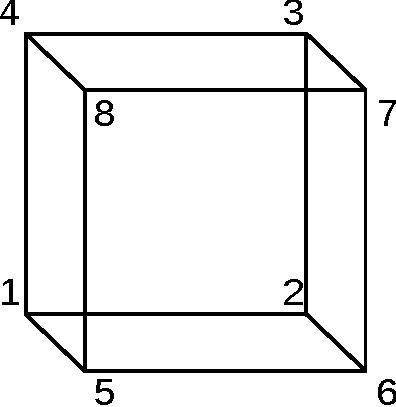
\includegraphics[height=0.25\textwidth]{doc/hex_ordering}
  \caption{Hexahedron node ordering used by libsupermesh, as used in
           Gmsh 2.12 (\url{http://gmsh.info/}).}\label{fig:hex_ordering}
\end{centering}\end{figure}

\noindent Tetrahedron-polyhedron intersection.

\begin{lstlisting}[language=FORTRAN]
  interface intersect_polys
    module procedure intersect_tet_planes
  end interface intersect_polys
\end{lstlisting}
  
\begin{lstlisting}[language=FORTRAN]
  pure subroutine intersect_tet_planes(tet_a, planes_b, tets_c, n_tets_c, vol_b, work)
    type(tet_type), intent(in) :: tet_a
    type(plane_type), dimension(:), intent(in)  :: planes_b
    type(tet_type), dimension(:), intent(inout) :: tets_c
    integer, intent(out) :: n_tets_c
    real, optional, intent(in) :: vol_b
    type(tet_type), dimension(:), target, optional, intent(inout) :: work
\end{lstlisting}

\begin{description}[font=\ttfamily\bfseries,leftmargin=2.2\parindent,labelindent=1.7\parindent,noitemsep]
  \item[tet\_a] Element A.
  \item[planes\_b] Element B facet half-spaces. Element B must be a convex
    polyhedron.
  \item[tets\_c] Length $M_C$ vector. Tetrahedra in mesh C.
  \item[n\_tets\_c] $E_C$.
  \item[vol\_b] Volume of element $B$. Used to discard near-degenerate elements
    in mesh C.
  \item[work] Length $M_C$ vector. Working memory.
\end{description}

\noindent Tetrahedron volume.

\begin{lstlisting}[language=FORTRAN]
  interface tetrahedron_volume
    module procedure tetrahedron_volume_real, tetrahedron_volume_tet
  end interface tetrahedron_volume
\end{lstlisting}

\begin{lstlisting}[language=FORTRAN]
  pure function tetrahedron_volume_real(tet) result(volume)
    real, dimension(3, 4), intent(in) :: tet
    real :: volume
\end{lstlisting}

\begin{description}[font=\ttfamily\bfseries,leftmargin=2.2\parindent,labelindent=1.7\parindent,noitemsep]
  \item[tet] $d \times l$ array. Tetrahedron node coordinates.
  \item[volume] Volume of the tetrahedron.
\end{description}

\begin{lstlisting}[language=FORTRAN]
  pure elemental function tetrahedron_volume_tet(tet) result(volume)
    type(tet_type), intent(in) :: tet
    real :: volume
\end{lstlisting}

\begin{description}[font=\ttfamily\bfseries,leftmargin=2.2\parindent,labelindent=1.7\parindent,noitemsep]
  \item[tet] A tetrahedron.
  \item[volume] Volume of the tetrahedron.
\end{description}

\subsection{General dimensions}\label{sect:nD_intersection}

Definition of $M_C$ for simplex-simplex intersection in one, two, and three
dimensions.

\begin{lstlisting}[language=FORTRAN]
  interface max_n_simplices_c
    module procedure max_n_simplices_c_simplices
  end interface max_n_simplices_c
\end{lstlisting}

\begin{lstlisting}[language=FORTRAN]
  pure elemental function max_n_simplices_c_simplices(dim) result(size)
    integer, intent(in) :: dim
    integer :: size
\end{lstlisting}

\begin{description}[font=\ttfamily\bfseries,leftmargin=2.2\parindent,labelindent=1.7\parindent,noitemsep]
  \item[dim] Dimension $d$. Must be equal to $1$, $2$, or $3$.
  \item[size] $M_C$. Equal to $1$ for the interval-interval case, $22$ for the
    triangle-triangle case, and $81$ for the tetrahedron-tetrahedron case.
\end{description}

\noindent Definition of $M_C$ for simplex-simplex, simplex-cubical, and
cubical-cubical intersection in one, two, and three dimensions.
  
\begin{lstlisting}[language=FORTRAN]
  interface max_n_simplices_c
    module procedure max_n_simplices_c_elements
  end interface max_n_simplices_c
\end{lstlisting}

\begin{lstlisting}[language=FORTRAN]
  pure elemental function max_n_simplices_c_elements(dim, loc_a, loc_b) result(size)
    integer, intent(in) :: dim
    integer, intent(in) :: loc_a
    integer, intent(in) :: loc_b
    integer :: size
\end{lstlisting}

\begin{description}[font=\ttfamily\bfseries,leftmargin=2.2\parindent,labelindent=1.7\parindent,noitemsep]
  \item[dim] Dimension $d$. Must be equal to $1$, $2$, or $3$.
  \item[loc\_a] $l_A$.
  \item[loc\_b] $l_B$.
  \item[size] $M_C$. Equal to \verb+max_n_simplices_c(dim)+ for the
    simplex-simplex case, $46$ for the \linebreak triangle-quadrilateral case,
    $62$ for the quadrilateral-quadrilateral case, $729$ for the \linebreak
    tetrahedron-hexahedron case, and $3,645$ for the hexahedron-hexahedron case.
\end{description}

\noindent Simplex-simplex intersection in one, two, and three dimensions.

\begin{lstlisting}[language=FORTRAN]
  subroutine intersect_simplices(simplex_a, simplex_b, &
    & simplices_c, n_simplices_c)
    real, dimension(:, :), intent(in) :: simplex_a
    real, dimension(:, :), intent(in) :: simplex_b
    real, dimension(:, :, :), intent(inout) :: simplices_c
    integer, intent(out) :: n_simplices_c
\end{lstlisting}

\begin{description}[font=\ttfamily\bfseries,leftmargin=2.2\parindent,labelindent=1.7\parindent,noitemsep]
  \item[simplex\_a, simplex\_b] $d \times l_A$ and $d \times l_B$ arrays.
    Element A and B node coordinates. Each element must be a one, two, or three
    dimensional simplex.
  \item[simplex\_c] $d \times l_C \times M_C$ array. Mesh C node coordinates.
  \item[n\_simplices\_c] $E_C$.
\end{description}

\noindent Simplex-simplex, simplex-cubical, and cubical-cubical
intersection in one, two, and three dimensions.

\begin{lstlisting}[language=FORTRAN]
  subroutine intersect_elements(element_a, element_b, elements_c, nelements_c)
    real, dimension(:, :), intent(in) :: element_a
    real, dimension(:, :), intent(in) :: element_b
    real, dimension(:, :, :), intent(inout) :: elements_c
    integer, intent(out) :: nelements_c
\end{lstlisting}

\begin{description}[font=\ttfamily\bfseries,leftmargin=2.2\parindent,labelindent=1.7\parindent,noitemsep]
  \item[element\_a, element\_b] $d \times l_A$ and $d \times l_B$ arrays.
    Element A and B node coordinates. See \verb+intersect_simplices+,
    \verb+intersect_tri_quad+, \verb+intersect_tet_hex+, \verb+intersect_quads+,
    and \verb+intersect_hexes+ for input requirements.
  \item[elements\_c] $d \times l_C \times M_C$ array. Mesh C node coordinates.
  \item[n\_simplices\_c] $E_C$.
\end{description}

\noindent Simplex volume in one, two, and three dimensions.

\begin{lstlisting}[language=FORTRAN]
  pure function simplex_volume(simplex) result(volume)
    real, dimension(:, :), intent(in) :: simplex
    real :: volume
\end{lstlisting}

\begin{description}[font=\ttfamily\bfseries,leftmargin=2.2\parindent,labelindent=1.7\parindent,noitemsep]
  \item[simplex] $d \times l$ array. Simplex node coordinates. Must be
    coordinates for a one, two, or three dimensional simplex.
  \item[volume] Simplex volume.
\end{description}

\section{Parallelisation}

libsupermesh provides a high-level interface for performing parallel supermesh
calculations, for the case where the domain decomposition of the two meshes A
and B do not match. 

In the following the local mesh A refers to the local submesh (or partition) of
mesh A stored on the current MPI process. Similarly the local mesh B refers to
the local submesh (or partition) of mesh B stored on the current MPI process.
The received mesh B refers to a submesh of mesh B received from a different MPI
process.

Candidate intersection identification is performed using the libspatialindex
R${}^*$-tree described in section \ref{sect:rtree_query}, and element
intersections are performed using the \verb+intersect_elements+ routine
described in section \ref{sect:nD_intersection}. Parallel communication is
performed using MPI.

The following definitions are used:
\begin{description}[leftmargin=\parindent,labelindent=\parindent]
  \item[$d$] Mesh A defines a subset $\Omega_A \subset \mathbb{R}^d$, and mesh B
    a subset $\Omega_B \subset \mathbb{R}^d$.
  \item[$V_A$] Number of nodes in the local mesh A.
  \item[$V_B$] Number of nodes in the local mesh B.
  \item[$E_A$] Number of elements in the local mesh A.
  \item[$E_B$] Number of elements in the local mesh B.
  \item[$V_B^*$] Number of nodes in a received mesh B.
  \item[$E_B^*$] Number of elements in a received mesh B.
  \item[$l_A$] Number of nodes per element in mesh A.
  \item[$l_B$] Number of nodes per element in mesh B.
  \item[$l_C$] Number of nodes per element in the intersection mesh C, always
               equal to $d + 1$.
  \item[$E_C$] Number of elements in the intersection mesh C.
\end{description}

\subsection{Algorithm}

The algorithm used is as follows:
\begin{enumerate}
  \item Communicate the AABBs of all mesh A partitions and all mesh B partitions
        using all-to-all communication
  \item For each mesh A partition whose AABB intersects with the local mesh B
        AABB
  \begin{enumerate}
    \item Identify local mesh B elements whose AABBs intersect with the AABB of
          the mesh A partition
    \item \label{alg:comm} Obtain data associated with these elements, and
          communicate these data via point-to-point communication
  \end{enumerate}
  \item Construct the intersection mesh for each pair of intersecting local
        mesh A and local mesh B elements, and perform calculations on these
        intersection meshes
  \item For each mesh B partition whose AABB intersects with the local mesh A
        AABB
  \begin{enumerate}
    \item Unpack data communicated in step \ref{alg:comm}
    \item Construct the intersection mesh for each pair of intersecting local
          mesh A and received mesh B elements, and perform calculations on these 
          intersection meshes
  \end{enumerate}
\end{enumerate}  

\subsection{\texttt{parallel\_supermesh}}

The parallel supermeshing interface accepts the local meshes, local mesh
element ownership information, and three callbacks. The interface optionally
accepts an MPI communicator.

\begin{lstlisting}[language=FORTRAN]
  subroutine parallel_supermesh(positions_a, enlist_a, ele_owner_a, &
    & positions_b, enlist_b, ele_owner_b, &
    & pack_data_b, unpack_data_b, intersection_calculation, &
    & comm)
    real, dimension(:, :), intent(in) :: positions_a
    integer, dimension(:, :), intent(in) :: enlist_a
    integer, dimension(:), intent(in) :: ele_owner_a
    real, dimension(:, :), intent(in) :: positions_b
    integer, dimension(:, :), intent(in) :: enlist_b
    integer, dimension(:), intent(in) :: ele_owner_b
    integer, optional, intent(in) :: comm
    
    interface
      subroutine pack_data_b(nodes_b, eles_b, data_b)
        use iso_c_binding, only : c_int8_t
        integer, dimension(:), intent(in) :: nodes_b
        integer, dimension(:), intent(in) :: eles_b
        integer(kind = c_int8_t), dimension(:), allocatable, intent(out) :: &
          & data_b
      end subroutine pack_data_b

      subroutine unpack_data_b(nnodes_b, nelements_b, data_b)
        use iso_c_binding, only : c_int8_t
        integer, intent(in) :: nnodes_b
        integer, intent(in) :: nelements_b
        integer(kind = c_int8_t), dimension(:), intent(in) :: data_b
      end subroutine unpack_data_b
      
      subroutine intersection_calculation(element_a, element_b, elements_c, &
        & nodes_b, ele_a, ele_b, local)
        real, dimension(:, :), intent(in) :: element_a
        real, dimension(:, :), intent(in) :: element_b
        real, dimension(:, :, :), intent(in) :: elements_c
        integer, dimension(:), intent(in) :: nodes_b
        integer, intent(in) :: ele_a
        integer, intent(in) :: ele_b
        logical, intent(in) :: local
      end subroutine intersection_calculation
    end interface
\end{lstlisting}

\begin{description}[font=\ttfamily\bfseries,leftmargin=2.2\parindent,labelindent=1.7\parindent,noitemsep]
  \item[positions\_a] $d \times V_A$ array. Local mesh A node coordinates.
  \item[enlist\_a] $l_A \times E_A$ array. Local mesh A element-node graph.
  \item[ele\_owner\_a] Length $E_A$ vector. MPI rank (indexed from zero) of the
    process which owns each element in the local mesh A.
  \item[positions\_b] $d \times V_B$ array. Local mesh B node coordinates.
  \item[enlist\_b] $l_B \times E_B$ array. Local mesh B element-node graph.
  \item[ele\_owner\_b] Length $E_B$ vector. MPI rank (indexed from zero) of the
    process which owns each element in the local mesh B.
  \item[pack\_data\_b, unpack\_data\_b, intersection\_calculation] Callbacks
    used to pack and unpack mesh B data, and to perform calculations on
    intersection meshes. See section \ref{sect:parallel_callbacks}.
  \item[comm] MPI communicator.
\end{description}

\subsection{Callbacks}\label{sect:parallel_callbacks}

\noindent The first callback is used to pack mesh B data for communication.

\begin{lstlisting}[language=FORTRAN]
  subroutine pack_data_b(nodes_b, eles_b, data_b)
    use iso_c_binding, only : c_int8_t
    integer, dimension(:), intent(in) :: nodes_b
    integer, dimension(:), intent(in) :: eles_b
    integer(kind = c_int8_t), dimension(:), allocatable, intent(out) :: data_b
\end{lstlisting}

\begin{description}[font=\ttfamily\bfseries,leftmargin=2.2\parindent,labelindent=1.7\parindent,noitemsep]
  \item[nodes\_b] The mesh B nodes to be communicated.
  \item[eles\_b] The mesh B elements to be communicated.
  \item[data\_b] Mesh B data to be communicated. This should consist of all
    data which will later be required by the \verb+intersection_calculation+
    callback, excluding the mesh node coordinates, and node and element indices.
\end{description}

\noindent The second callpack unpacks these data.

\begin{lstlisting}[language=FORTRAN]
  subroutine unpack_data_b(nnodes_b, nelements_b, data_b)
    use iso_c_binding, only : c_int8_t
    integer, intent(in) :: nnodes_b
    integer, intent(in) :: nelements_b
    integer(kind = c_int8_t), dimension(:), intent(in) :: data_b
\end{lstlisting}

\begin{description}[font=\ttfamily\bfseries,leftmargin=2.2\parindent,labelindent=1.7\parindent,noitemsep]
  \item[nodes\_b] $V_B^*$.
  \item[eles\_b] $E_B^*$.
  \item[data\_b] Received mesh B data, previously packed on a different process
    using \verb+pack_data_b+.
\end{description}

\noindent The final callback performs calculations on each intersection mesh.
      
\begin{lstlisting}[language=FORTRAN]
  subroutine intersection_calculation(element_a, element_b, elements_c, &
    & nodes_b, ele_a, ele_b, local)
    real, dimension(:, :), intent(in) :: element_a
    real, dimension(:, :), intent(in) :: element_b
    real, dimension(:, :, :), intent(in) :: elements_c
    integer, dimension(:), intent(in) :: nodes_b
    integer, intent(in) :: ele_a
    integer, intent(in) :: ele_b
    logical, intent(in) :: local
\end{lstlisting}

\begin{description}[font=\ttfamily\bfseries,leftmargin=2.2\parindent,labelindent=1.7\parindent,noitemsep]
  \item[element\_a] $d \times l_A$ array. Element A node coordinates.
  \item[element\_b] $d \times l_B$ array. Element B node coordinates.
  \item[elements\_c] $d \times l_C \times E_C$. Intersection mesh C node
    coordinates.
  \item[nodes\_b] Length $l_B$ vector. If \verb+local+ is true, local mesh B
    nodes associated with element B. If \verb+local+ is false, received mesh B
    nodes associated with element B.
  \item[ele\_a] Index of element A in the local mesh A.
  \item[ele\_b] If \verb+local+ is true, index of element B in the local mesh B.
    If \verb+local+ is false, index of element B in the received mesh B.
  \item[local] If \verb+local+ is true then the calculation involves the local
    mesh B. If \verb+local+ is false then the calculation involves the received
    mesh B.
\end{description}

\section{Examples}

\subsection{Serial}\label{sect:serial_example}

In this example two triangle meshes A and B, possibly covering differing domains
$\Omega_A$ and $\Omega_B$, are considered, and their area of intersection is
computed.

libsupermesh requires that the calling code set up all relevant mesh data.
However for internal testing purposes libsupermesh includes the \verb+read_node+
and \verb+read_ele+ routines which can be used to read files which are in
Triangle\footnote{\url{https://www.cs.cmu.edu/~quake/triangle.html}} or
TetGen\footnote{\url{http://wias-berlin.de/software/tetgen/}} .node and .ele
format (with some generalisation to allow cubical mesh input). Note that these
additional routines are not included in the \verb+libsupermesh+ Fortran module.

~\newline
First the necessary libsupermesh library functionality is accessed.
\begin{lstlisting}[language=FORTRAN]
program serial_example

  use libsupermesh, only : quadtree_type, allocate, query, deallocate
  use libsupermesh, only : tri_buf_size, intersect_tris, triangle_area
  use libsupermesh_read_triangle, only : read_node, read_ele

  implicit none
\end{lstlisting}

~\newline
Variables are defined.
\begin{lstlisting}[language=FORTRAN]
  real, dimension(:, :), allocatable :: positions_a, positions_b
  integer, dimension(:, :), allocatable :: enlist_a, enlist_b
  integer :: nnodes_a, nnodes_b, nelements_a
  
  type(quadtree_type) :: tree
  integer :: ele_a, i_eles_b
  integer, dimension(:), allocatable :: eles_b
  
  real, dimension(2, 3) :: tri_a, tri_b
  real, dimension(2, 3, tri_buf_size) :: tris_c
  integer :: n_tris_c, ele_c
  
  real :: area
\end{lstlisting}

~\newline
The mesh node coordinates and element-node graphs are read.
\begin{lstlisting}[language=FORTRAN]
  ! Read mesh A data
  call read_node('square_0_01.node', dim = 2, positions = positions_a)
  call read_ele('square_0_01.ele', dim = 2, enlist = enlist_a)
  nnodes_a = size(positions_a, 2)
  nelements_a = size(enlist_a, 2)
  
  ! Read mesh B data
  call read_node('triangle_0_01.node', dim = 2, positions = positions_b)
  call read_ele('triangle_0_01.ele', dim = 2, enlist = enlist_b)
  nnodes_b = size(positions_b, 2)
\end{lstlisting}

~\newline
In the following a quadtree is constructed, and successively
queried for candidate intersecting mesh B elements, using mesh A element node
coordinates (see section \ref{sect:quadtree_query}). These are used to construct
(possibly empty) intersection meshes. The intersection area is added to
\verb+area+.
\begin{lstlisting}[language=FORTRAN]
  ! Build a quadtree
  call allocate(tree, positions_b, enlist_b)
  
  area = 0.0D0
  do ele_a = 1, nelements_a
    tri_a = positions_a(:, enlist_a(:, ele_a))
    ! Query the quadtree for candidate intersecting elements
    call query(tree, tri_a, eles_b)
    do i_eles_b = 1, size(eles_b)
      tri_b = positions_b(:, enlist_b(:, eles_b(i_eles_b)))
      ! Construct an intersection mesh
      call intersect_tris(tri_a, tri_b, tris_c, n_tris_c)
      do ele_c = 1, n_tris_c
        ! Add the area of the intersection mesh element
        area = area + triangle_area(tris_c(:, :, ele_c))
      end do
    end do
  end do
\end{lstlisting}

~\newline
Finally the result is displayed, and necessary deallocation is performed.
\begin{lstlisting}[language=FORTRAN]    
  ! Display the result
  print '(a,e26.18e3)', 'Area of intersection = ', area
  
  ! Deallocation
  call deallocate(tree)
  deallocate(positions_a, enlist_a, positions_b, enlist_b)
  
end program serial_example
\end{lstlisting}

~\newline
The complete code.
\begin{lstlisting}[language=FORTRAN]
program serial_example

  use libsupermesh, only : quadtree_type, allocate, query, deallocate
  use libsupermesh, only : tri_buf_size, intersect_tris, triangle_area
  use libsupermesh_read_triangle, only : read_node, read_ele

  implicit none
  
  real, dimension(:, :), allocatable :: positions_a, positions_b
  integer, dimension(:, :), allocatable :: enlist_a, enlist_b
  integer :: nnodes_a, nnodes_b, nelements_a
  
  type(quadtree_type) :: tree
  integer :: ele_a, i_eles_b
  integer, dimension(:), allocatable :: eles_b
  
  real, dimension(2, 3) :: tri_a, tri_b
  real, dimension(2, 3, tri_buf_size) :: tris_c
  integer :: n_tris_c, ele_c
  
  real :: area
  
  ! Read mesh A data
  call read_node('square_0_01.node', dim = 2, positions = positions_a)
  call read_ele('square_0_01.ele', dim = 2, enlist = enlist_a)
  nnodes_a = size(positions_a, 2)
  nelements_a = size(enlist_a, 2)
  
  ! Read mesh B data
  call read_node('triangle_0_01.node', dim = 2, positions = positions_b)
  call read_ele('triangle_0_01.ele', dim = 2, enlist = enlist_b)
  nnodes_b = size(positions_b, 2)
  
  ! Build a quadtree
  call allocate(tree, positions_b, enlist_b)
  
  area = 0.0D0
  do ele_a = 1, nelements_a
    tri_a = positions_a(:, enlist_a(:, ele_a))
    ! Query the quadtree for candidate intersecting elements
    call query(tree, tri_a, eles_b)
    do i_eles_b = 1, size(eles_b)
      tri_b = positions_b(:, enlist_b(:, eles_b(i_eles_b)))
      ! Construct an intersection mesh
      call intersect_tris(tri_a, tri_b, tris_c, n_tris_c)
      do ele_c = 1, n_tris_c
        ! Add the area of the intersection mesh element
        area = area + triangle_area(tris_c(:, :, ele_c))
      end do
    end do
  end do
  
  ! Display the result
  print '(a,e26.18e3)', 'Area of intersection = ', area
  
  ! Deallocation
  call deallocate(tree)
  deallocate(positions_a, enlist_a, positions_b, enlist_b)
  
end program serial_example
\end{lstlisting}

\subsection{Parallel}

In this example two triangle meshes A and B, possibly covering differing domains
$\Omega_A$ and $\Omega_B$ and partitioned for an MPI calculation, are
considered. A $C^0$ real function $\phi_B$ which is piecewise linear within the
elements of mesh B is defined (a $P_1$ function on mesh B), and the integral
over the intersection region,
\begin{equation*}
  I = \int_{\Omega_A \cap \Omega_B} \phi_B,
\end{equation*}
is computed.

libsupermesh requires that the calling code set up all relevant mesh and element
ownership data. Here local mesh data are read as described in section
\ref{sect:serial_example}. For internal testing purposes libsupermesh includes
routines for reading Fluidity .halo files, which define node ownership in an
overlap ``halo'' (or ``ghost'') region. libsupermesh similarly includes, for
testing purposes, the routine \verb+element_ownership+, which can be used to
generate consistent element ownership information from these halo data. Note
that these additional routines are not included in the \verb+libsupermesh+
Fortran module.

In this example packing and unpacking of additional data, via the
\verb+pack_data_b+ and \linebreak \verb+unpack_data_b+ callbacks, could be
avoided by swapping the roles of meshes A and B. Here this arrangement is
retained in order to illustrate the principles of packing and unpacking data in
parallel supermeshing.

~\newline
First necessary Fortran modules are used.
\begin{lstlisting}[language=FORTRAN]
program parallel_example

  use iso_c_binding, only : c_int8_t
  use iso_fortran_env, only : output_unit, error_unit
  use mpi
  
  use libsupermesh, only : parallel_supermesh, triangle_area
  use libsupermesh_halo_ownership, only : element_ownership
  use libsupermesh_read_halos, only : halo_type, read_halo, deallocate
  use libsupermesh_read_triangle, only : read_node, read_ele

  implicit none
\end{lstlisting}

~\newline
Variables are defined.
\begin{lstlisting}[language=FORTRAN]
  character(len = int(log10(real(huge(0)))) + 2) :: rank_chr
  integer :: ierr, rank, real_extent
  
  real, dimension(:, :), allocatable :: positions_a, positions_b
  integer, dimension(:, :), allocatable :: enlist_a, enlist_b
  integer :: nnodes_b, nelements_a, nelements_b
  real, dimension(:), allocatable, target :: phi_b
  
  type(halo_type) :: halo
  integer, dimension(:), allocatable :: ele_owner_a, ele_owner_b
  
  real, dimension(:), allocatable, target :: phi_b_received
  
  real :: integral
\end{lstlisting}

~\newline
MPI is initialised, and the extent of MPI double precision variables is
determined. The extent will later be used to faciliate packing and unpacking of
data for parallel supermeshing.
\begin{lstlisting}[language=FORTRAN]
  call MPI_Init(ierr)
  if(ierr /= MPI_SUCCESS) stop 1
  
  ! Find the extent of a double precision variable
  call MPI_Type_extent(MPI_DOUBLE_PRECISION, real_extent, ierr)
  if(ierr /= MPI_SUCCESS) call MPI_Abort(MPI_COMM_WORLD, MPI_ERR_OTHER, ierr)
\end{lstlisting}

~\newline
The mesh node coordinates and element-node graphs are read, and element
ownership is determined by reading halo data.
\begin{lstlisting}[language=FORTRAN]    
  ! Find the process rank, and convert to a string
  call MPI_Comm_rank(MPI_COMM_WORLD, rank, ierr)
  if(ierr /= MPI_SUCCESS) call MPI_Abort(MPI_COMM_WORLD, MPI_ERR_OTHER, ierr)
  write(rank_chr, '(i0)') rank
  rank_chr = adjustl(rank_chr)
  
  ! Read mesh A data
  call read_node('square_0_01_4_' // trim(rank_chr) // '.node', dim = 2, &
    & positions = positions_a)
  call read_ele('square_0_01_4_' // trim(rank_chr) // '.ele', dim = 2, &
    & enlist = enlist_a)
  nelements_a = size(enlist_a, 2)
    
  ! Read mesh A halo data, and construct element ownership
  call read_halo('square_0_01_4', halo, level = 2)
  allocate(ele_owner_a(nelements_a))
  call element_ownership(size(positions_a, 2), enlist_a, halo, ele_owner_a)
  call deallocate(halo)
    
  ! Read mesh B data
  call read_node('triangle_0_01_4_' // trim(rank_chr) // '.node', dim = 2, &
    & positions = positions_b)
  call read_ele('triangle_0_01_4_' // trim(rank_chr) // '.ele', dim = 2, &
    & enlist = enlist_b)
  nnodes_b = size(positions_b, 2)
  nelements_b = size(enlist_b, 2)
    
  ! Read mesh B halo data, and construct element ownership
  call read_halo('triangle_0_01_4', halo, level = 2)
  allocate(ele_owner_b(nelements_b))
  call element_ownership(size(positions_b, 2), enlist_b, halo, ele_owner_b)
  call deallocate(halo)
\end{lstlisting}

~\newline
Nodal data for $\phi_B$ are constructed. Here $\phi_B$ is set equal to the value
of the $x$-coordinate. The vector \verb+phi_b+ contains the values of $\phi_B$
on the mesh nodes.
\begin{lstlisting}[language=FORTRAN]
  ! Construct a P1 field on mesh B
  allocate(phi_b(nnodes_b))
  phi_b = positions_b(1, :)
\end{lstlisting}

~\newline
Parallel supermeshing is used to compute the integral over the local mesh A.
The callbacks and the \verb+cleanup_data_b+ routine are described below.
\begin{lstlisting}[language=FORTRAN]
  ! Compute the integral over the local mesh A
  integral = 0.0D0
  call parallel_supermesh(positions_a, enlist_a, ele_owner_a, &
     & positions_b, enlist_b, ele_owner_b, &
     & pack_data_b, unpack_data_b, intersection_calculation, &
     & comm = MPI_COMM_WORLD)
  call cleanup_data_b()
\end{lstlisting}

~\newline
The integral over the whole of mesh A is computed using \verb+MPI_Allreduce+.
\begin{lstlisting}[language=FORTRAN]  
  ! Compute the total integral over mesh A
  call MPI_Allreduce(MPI_IN_PLACE, integral, 1, MPI_DOUBLE_PRECISION, &
    & MPI_SUM, MPI_COMM_WORLD, ierr)
  if(ierr /= MPI_SUCCESS) call MPI_Abort(MPI_COMM_WORLD, MPI_ERR_OTHER, ierr)
\end{lstlisting}

~\newline
Finally the result is displayed, and necessary deallocation and MPI finalisation
is performed.
\begin{lstlisting}[language=FORTRAN]  
  ! Display the result
  flush(output_unit)
  flush(error_unit)
  call MPI_Barrier(MPI_COMM_WORLD, ierr)
  if(ierr /= MPI_SUCCESS) call MPI_Abort(MPI_COMM_WORLD, MPI_ERR_OTHER, ierr)
  if(rank == 0) print '(a,e26.18e3)', 'Integral = ', integral
  flush(output_unit)
  flush(error_unit)
      
  ! Deallocation
  deallocate(positions_a, enlist_a, positions_b, enlist_b, &
    & ele_owner_a, ele_owner_b, phi_b)
  
  call MPI_Finalize(ierr)
  if(ierr /= MPI_SUCCESS) stop 1
\end{lstlisting}

~\newline
The first callback packs the $P_1$ nodal data used to represent $\phi_B$ using
\verb+MPI_Pack+. Note that, since the ordering of degree-of-freedom data in
\verb+phi_b+ is consistent with the ordering of nodes in \verb+positions_b+, no
degree-of-freedom ordering information need be packed
here.
\begin{lstlisting}[language=FORTRAN]  
contains

  subroutine pack_data_b(nodes_b, eles_b, data_b)
    integer, dimension(:), intent(in) :: nodes_b
    integer, dimension(:), intent(in) :: eles_b
    integer(kind = c_int8_t), dimension(:), allocatable, intent(out) :: data_b

    integer :: ierr, ndata_b, position
    real, dimension(:), allocatable :: ldata

    ! Extract nodal data to be communicated
    allocate(ldata(size(nodes_b)))
    ldata = phi_b(nodes_b)

    ! Pack data for sending
    ndata_b = size(nodes_b) * real_extent
    allocate(data_b(ndata_b))
    position = 0
    call MPI_Pack(ldata, size(nodes_b), MPI_DOUBLE_PRECISION, data_b, ndata_b, &
      & position, MPI_COMM_WORLD, ierr)
    if(ierr /= MPI_SUCCESS) call MPI_Abort(MPI_COMM_WORLD, MPI_ERR_OTHER, ierr)

    ! Deallocation
    deallocate(ldata)
    
  end subroutine pack_data_b
\end{lstlisting}

~\newline
The second callback unpacks received mesh B data using \verb+MPI_Unpack+. The
additional routine \verb+cleanup_data_b+ is used to deallocate any previously
unpacked data. Note that \verb+cleanup_data_b+ is also called after the
\verb+parallel_supermesh+ call above.
\begin{lstlisting}[language=FORTRAN] 
  subroutine unpack_data_b(nnodes_b, nelements_b, data_b)
    integer, intent(in) :: nnodes_b
    integer, intent(in) :: nelements_b
    integer(kind = c_int8_t), dimension(:), intent(in) :: data_b

    integer :: ierr, position

    ! Deallocate any previously unpacked data
    call cleanup_data_b()

    ! Unpack received data
    allocate(phi_b_received(nnodes_b))
    position = 0
    call MPI_Unpack(data_b, size(data_b), position, phi_b_received, nnodes_b, &
      & MPI_DOUBLE_PRECISION, MPI_COMM_WORLD, ierr)
    if(ierr /= MPI_SUCCESS) call MPI_Abort(MPI_COMM_WORLD, MPI_ERR_OTHER, ierr)

  end subroutine unpack_data_b 

  ! Deallocate any previously unpacked data
  subroutine cleanup_data_b()
    if(allocated(phi_b_received)) deallocate(phi_b_received)
  end subroutine cleanup_data_b
\end{lstlisting}

~\newline
The final callback performs calculations on the intersection mesh. Two utility
functions are defined, which are used to interpolate $P_1$ nodal data onto an
arbitrary point (using Lagrange basis functions).
\begin{lstlisting}[language=FORTRAN] 
  ! Evaluate P1 basis functions at a given point
  pure function basis_functions_p1(element, coord) result(fns)
    real, dimension(2, 3), intent(in) :: element
    real, dimension(2), intent(in) :: coord

    real, dimension(3) :: fns

    real, dimension(2) :: e1, e2
    real, dimension(2, 2) :: jac
        
    e1 = element(:, 2) - element(:, 1)
    e2 = element(:, 3) - element(:, 1)

    jac(1, 1) =  e2(2);  jac(1, 2) = -e2(1)
    jac(2, 1) = -e1(2);  jac(2, 2) =  e1(1)
    jac = jac / (jac(1, 1) * jac(2, 2) - jac(1, 2) * jac(2, 1))

    fns(2:3) = matmul(jac, coord - element(:, 1))
    fns(1) = 1.0D0 - fns(2) - fns(3)

  end function basis_functions_p1

  ! Interpolate a P1 function at given point
  pure function interpolate_p1(element, phi, coord) result(phi_c)
    real, dimension(2, 3), intent(in) :: element
    real, dimension(3), intent(in) :: phi
    real, dimension(2), intent(in) :: coord

    real :: phi_c

    phi_c = dot_product(basis_functions_p1(element, coord), phi)

  end function interpolate_p1
\end{lstlisting}
The callback itself computes an intergal over each intersection mesh C using
degree one quadrature. The \verb+local+ argument is used to determine if local
mesh B data, \verb+phi_b+, or received mesh B data,
\verb+phi_b_received+, should be used in this calculation.
\begin{lstlisting}[language=FORTRAN] 
  subroutine intersection_calculation(element_a, element_b, elements_c, &
    & nodes_b, ele_a, ele_b, local)
    real, dimension(:, :), intent(in) :: element_a
    real, dimension(:, :), intent(in) :: element_b
    real, dimension(:, :, :), intent(in) :: elements_c
    integer, dimension(:), intent(in) :: nodes_b
    integer, intent(in) :: ele_a
    integer, intent(in) :: ele_b
    logical, intent(in) :: local

    integer :: ele_c, nelements_c
    real, dimension(:), pointer :: lphi_b
    
    if(local) then
      ! If calculations are being performed using the local mesh B, use the
      ! local field data
      lphi_b => phi_b
    else
      ! Otherwise use previously unpacked received field data
      lphi_b => phi_b_received
    end if

    nelements_c = size(elements_c, 3)
    do ele_c = 1, nelements_c
      ! Add the integral over an intersection element using one-point quadrature
      integral = integral + &
        & interpolate_p1(element_b, lphi_b(nodes_b), &
          & sum(elements_c(:, :, ele_c), 2) / 3.0D0) &
        & * triangle_area(elements_c(:, :, ele_c))
    end do    
    
  end subroutine intersection_calculation
  
end program parallel_example
\end{lstlisting}

~\newline
The complete code.
\begin{lstlisting}[language=FORTRAN]
program parallel_example

  use iso_c_binding, only : c_int8_t
  use iso_fortran_env, only : output_unit, error_unit
  use mpi
  
  use libsupermesh, only : parallel_supermesh, triangle_area
  use libsupermesh_halo_ownership, only : element_ownership
  use libsupermesh_read_halos, only : halo_type, read_halo, deallocate
  use libsupermesh_read_triangle, only : read_node, read_ele

  implicit none
  
  character(len = int(log10(real(huge(0)))) + 2) :: rank_chr
  integer :: ierr, rank, real_extent
  
  real, dimension(:, :), allocatable :: positions_a, positions_b
  integer, dimension(:, :), allocatable :: enlist_a, enlist_b
  integer :: nnodes_b, nelements_a, nelements_b
  real, dimension(:), allocatable, target :: phi_b
  
  type(halo_type) :: halo
  integer, dimension(:), allocatable :: ele_owner_a, ele_owner_b
  
  real, dimension(:), allocatable, target :: phi_b_received
  
  real :: integral
  
  call MPI_Init(ierr)
  if(ierr /= MPI_SUCCESS) stop 1
  
  ! Find the extent of a double precision variable
  call MPI_Type_extent(MPI_DOUBLE_PRECISION, real_extent, ierr)
  if(ierr /= MPI_SUCCESS) call MPI_Abort(MPI_COMM_WORLD, MPI_ERR_OTHER, ierr)
  
  ! Find the process rank, and convert to a string
  call MPI_Comm_rank(MPI_COMM_WORLD, rank, ierr)
  if(ierr /= MPI_SUCCESS) call MPI_Abort(MPI_COMM_WORLD, MPI_ERR_OTHER, ierr)
  write(rank_chr, '(i0)') rank
  rank_chr = adjustl(rank_chr)
  
  ! Read mesh A data
  call read_node('square_0_01_4_' // trim(rank_chr) // '.node', dim = 2, &
    & positions = positions_a)
  call read_ele('square_0_01_4_' // trim(rank_chr) // '.ele', dim = 2, &
    & enlist = enlist_a)
  nelements_a = size(enlist_a, 2)
    
  ! Read mesh A halo data, and construct element ownership
  call read_halo('square_0_01_4', halo, level = 2)
  allocate(ele_owner_a(nelements_a))
  call element_ownership(size(positions_a, 2), enlist_a, halo, ele_owner_a)
  call deallocate(halo)
    
  ! Read mesh B data
  call read_node('triangle_0_01_4_' // trim(rank_chr) // '.node', dim = 2, &
    & positions = positions_b)
  call read_ele('triangle_0_01_4_' // trim(rank_chr) // '.ele', dim = 2, &
    & enlist = enlist_b)
  nnodes_b = size(positions_b, 2)
  nelements_b = size(enlist_b, 2)
    
  ! Read mesh B halo data, and construct element ownership
  call read_halo('triangle_0_01_4', halo, level = 2)
  allocate(ele_owner_b(nelements_b))
  call element_ownership(size(positions_b, 2), enlist_b, halo, ele_owner_b)
  call deallocate(halo)
    
  ! Construct a P1 field on mesh B
  allocate(phi_b(nnodes_b))
  phi_b = positions_b(1, :)
  
  ! Compute the integral over the local mesh A
  integral = 0.0D0
  call parallel_supermesh(positions_a, enlist_a, ele_owner_a, &
     & positions_b, enlist_b, ele_owner_b, &
     & pack_data_b, unpack_data_b, intersection_calculation, &
     & comm = MPI_COMM_WORLD)
  call cleanup_data_b()  
  
  ! Compute the total integral over mesh A
  call MPI_Allreduce(MPI_IN_PLACE, integral, 1, MPI_DOUBLE_PRECISION, &
    & MPI_SUM, MPI_COMM_WORLD, ierr)
  if(ierr /= MPI_SUCCESS) call MPI_Abort(MPI_COMM_WORLD, MPI_ERR_OTHER, ierr)

  ! Display the result
  flush(output_unit)
  flush(error_unit)
  call MPI_Barrier(MPI_COMM_WORLD, ierr)
  if(ierr /= MPI_SUCCESS) call MPI_Abort(MPI_COMM_WORLD, MPI_ERR_OTHER, ierr)
  if(rank == 0) print '(a,e26.18e3)', 'Integral = ', integral
  flush(output_unit)
  flush(error_unit)
      
  ! Deallocation
  deallocate(positions_a, enlist_a, positions_b, enlist_b, &
    & ele_owner_a, ele_owner_b, phi_b)
  
  call MPI_Finalize(ierr)
  if(ierr /= MPI_SUCCESS) stop 1

contains

  subroutine pack_data_b(nodes_b, eles_b, data_b)
    integer, dimension(:), intent(in) :: nodes_b
    integer, dimension(:), intent(in) :: eles_b
    integer(kind = c_int8_t), dimension(:), allocatable, intent(out) :: data_b

    integer :: ierr, ndata_b, position
    real, dimension(:), allocatable :: ldata

    ! Extract nodal data to be communicated
    allocate(ldata(size(nodes_b)))
    ldata = phi_b(nodes_b)

    ! Pack data for sending
    ndata_b = size(nodes_b) * real_extent
    allocate(data_b(ndata_b))
    position = 0
    call MPI_Pack(ldata, size(nodes_b), MPI_DOUBLE_PRECISION, data_b, ndata_b, &
      & position, MPI_COMM_WORLD, ierr)
    if(ierr /= MPI_SUCCESS) call MPI_Abort(MPI_COMM_WORLD, MPI_ERR_OTHER, ierr)

    ! Deallocation
    deallocate(ldata)
    
  end subroutine pack_data_b

  subroutine unpack_data_b(nnodes_b, nelements_b, data_b)
    integer, intent(in) :: nnodes_b
    integer, intent(in) :: nelements_b
    integer(kind = c_int8_t), dimension(:), intent(in) :: data_b

    integer :: ierr, position

    ! Deallocate any previously unpacked data
    call cleanup_data_b()

    ! Unpack received data
    allocate(phi_b_received(nnodes_b))
    position = 0
    call MPI_Unpack(data_b, size(data_b), position, phi_b_received, nnodes_b, &
      & MPI_DOUBLE_PRECISION, MPI_COMM_WORLD, ierr)
    if(ierr /= MPI_SUCCESS) call MPI_Abort(MPI_COMM_WORLD, MPI_ERR_OTHER, ierr)

  end subroutine unpack_data_b

  ! Deallocate any previously unpacked data
  subroutine cleanup_data_b()
    if(allocated(phi_b_received)) deallocate(phi_b_received)
  end subroutine cleanup_data_b
  
  ! Evaluate P1 basis functions at a given point
  pure function basis_functions_p1(element, coord) result(fns)
    real, dimension(2, 3), intent(in) :: element
    real, dimension(2), intent(in) :: coord

    real, dimension(3) :: fns

    real, dimension(2) :: e1, e2
    real, dimension(2, 2) :: jac
        
    e1 = element(:, 2) - element(:, 1)
    e2 = element(:, 3) - element(:, 1)

    jac(1, 1) =  e2(2);  jac(1, 2) = -e2(1)
    jac(2, 1) = -e1(2);  jac(2, 2) =  e1(1)
    jac = jac / (jac(1, 1) * jac(2, 2) - jac(1, 2) * jac(2, 1))

    fns(2:3) = matmul(jac, coord - element(:, 1))
    fns(1) = 1.0D0 - fns(2) - fns(3)

  end function basis_functions_p1

  ! Interpolate a P1 function at given point
  pure function interpolate_p1(element, phi, coord) result(phi_c)
    real, dimension(2, 3), intent(in) :: element
    real, dimension(3), intent(in) :: phi
    real, dimension(2), intent(in) :: coord

    real :: phi_c

    phi_c = dot_product(basis_functions_p1(element, coord), phi)

  end function interpolate_p1
  
  subroutine intersection_calculation(element_a, element_b, elements_c, &
    & nodes_b, ele_a, ele_b, local)
    real, dimension(:, :), intent(in) :: element_a
    real, dimension(:, :), intent(in) :: element_b
    real, dimension(:, :, :), intent(in) :: elements_c
    integer, dimension(:), intent(in) :: nodes_b
    integer, intent(in) :: ele_a
    integer, intent(in) :: ele_b
    logical, intent(in) :: local

    integer :: ele_c, nelements_c
    real, dimension(:), pointer :: lphi_b
    
    if(local) then
      ! If calculations are being performed using the local mesh B, use the
      ! local field data
      lphi_b => phi_b
    else
      ! Otherwise use previously unpacked received field data
      lphi_b => phi_b_received
    end if

    nelements_c = size(elements_c, 3)
    do ele_c = 1, nelements_c
      ! Add the integral over an intersection element using one-point quadrature
      integral = integral + &
        & interpolate_p1(element_b, lphi_b(nodes_b), &
          & sum(elements_c(:, :, ele_c), 2) / 3.0D0) &
        & * triangle_area(elements_c(:, :, ele_c))
    end do    
    
  end subroutine intersection_calculation
  
end program parallel_example
\end{lstlisting}

\section{Copyright}\label{sect:copyright}

\subsection{libsupermesh}

Except as noted below, libsupermesh is copyright \textcopyright\ 2016 The
University of Edinburgh. libsupermesh is available under the GNU Lesser General
Public License version 2.1, which can be found in lgpl-2.1.txt.

\begin{lstlisting}[language=]
  This library is free software; you can redistribute it and/or
  modify it under the terms of the GNU Lesser General Public
  License as published by the Free Software Foundation;
  version 2.1 of the License.

  This library is distributed in the hope that it will be useful,
  but WITHOUT ANY WARRANTY; without even the implied warranty of
  MERCHANTABILITY or FITNESS FOR A PARTICULAR PURPOSE.  See the GNU
  Lesser General Public License for more details.

  You should have received a copy of the GNU Lesser General Public
  License along with this library; if not, write to the Free Software
  Foundation, Inc., 51 Franklin Street, Fifth Floor, Boston, MA  02110-1301  USA
\end{lstlisting}

\subsection{Fluidity}

libsupermesh is derived from
Fluidity\footnote{\url{http://fluidityproject.github.io/}} git revision
4e6c1d2b022df3a519cdec120fad28e60d1b08d9 (dated 2015-02-25). libsupermesh
additionally uses code from Fluidity 4.1.11 -- see comments in src/Graphs.F90.
Fluidity copyright information (note that AUTHORS mentioned in the following has
been renamed to Fluidity\_AUTHORS):

\begin{lstlisting}[language=]
  Copyright (C) 2006 Imperial College London and others.
  
  Please see the AUTHORS file in the main source directory for a full list
  of copyright holders.

  Prof. C Pain
  Applied Modelling and Computation Group
  Department of Earth Science and Engineering
  Imperial College London

  amcgsoftware@imperial.ac.uk
  
  This library is free software; you can redistribute it and/or
  modify it under the terms of the GNU Lesser General Public
  License as published by the Free Software Foundation,
  version 2.1 of the License.

  This library is distributed in the hope that it will be useful,
  but WITHOUT ANY WARRANTY; without even the implied warranty of
  MERCHANTABILITY or FITNESS FOR A PARTICULAR PURPOSE.  See the GNU
  Lesser General Public License for more details.

  You should have received a copy of the GNU Lesser General Public
  License along with this library; if not, write to the Free Software
  Foundation, Inc., 59 Temple Place, Suite 330, Boston, MA  02111-1307
  USA
\end{lstlisting}

\subsection{TinyXML}

libsupermesh includes a modified version of
TinyXML\footnote{\url{http://www.grinninglizard.com/tinyxml/}} 2.6.2
(include/tinystr.h, include/tinyxml.h, \linebreak src/tinystr.cpp,
src/tinyxml.cpp, src/tinyxmlerror.cpp, src/tinyxmlparser.cpp, and
TinyXML\_readme.txt). Further information regarding TinyXML can be found in
TinyXML\_readme.txt. TinyXML 2.6.2 license information:

\begin{lstlisting}[language=]
  www.sourceforge.net/projects/tinyxml
  Original code by Lee Thomason (www.grinninglizard.com)

  This software is provided 'as-is', without any express or implied
  warranty. In no event will the authors be held liable for any
  damages arising from the use of this software.

  Permission is granted to anyone to use this software for any
  purpose, including commercial applications, and to alter it and
  redistribute it freely, subject to the following restrictions:

  1. The origin of this software must not be misrepresented; you must
  not claim that you wrote the original software. If you use this
  software in a product, an acknowledgment in the product documentation
  would be appreciated but is not required.

  2. Altered source versions must be plainly marked as such, and
  must not be misrepresented as being the original software.

  3. This notice may not be removed or altered from any source
  distribution.
\end{lstlisting}

\subsection{libspatialindex}

libsupermesh includes a modified version of
libspatialindex\footnote{\url{https://libspatialindex.github.io/}} 1.8.5
(in spatialindex-1.8.5/). libsupermesh additionally uses modified versions of
code from libspatialindex -- see comments in \linebreak
include/R-Tree\_Intersection\_Finder\_C++.h and
src/R-Tree\_Intersection\_Finder\_C++.cpp. Further information regarding
libspatialindex can be found in spatialindex-1.8.5/. libspatialindex 1.8.5
license information:

\begin{lstlisting}[language=]
License (MIT)
------------------------------------------------------------------------------

::

    Permission is hereby granted, free of charge, to any person obtaining a
    copy of this software and associated documentation files (the "Software"),
    to deal in the Software without restriction, including without limitation
    the rights to use, copy, modify, merge, publish, distribute, sublicense,
    and/or sell copies of the Software, and to permit persons to whom the
    Software is furnished to do so, subject to the following conditions:

    The above copyright notice and this permission notice shall be included in
    all copies or substantial portions of the Software.

    THE SOFTWARE IS PROVIDED "AS IS", WITHOUT WARRANTY OF ANY KIND, EXPRESS OR
    IMPLIED, INCLUDING BUT NOT LIMITED TO THE WARRANTIES OF MERCHANTABILITY,
    FITNESS FOR A PARTICULAR PURPOSE AND NONINFRINGEMENT. IN NO EVENT SHALL THE
    AUTHORS OR COPYRIGHT HOLDERS BE LIABLE FOR ANY CLAIM, DAMAGES OR OTHER
    LIABILITY, WHETHER IN AN ACTION OF CONTRACT, TORT OR OTHERWISE, ARISING
    FROM, OUT OF OR IN CONNECTION WITH THE SOFTWARE OR THE USE OR OTHER
    DEALINGS IN THE SOFTWARE.
\end{lstlisting}

\subsection{Rtree}

libsupermesh uses modified versions of code from
Rtree\footnote{\url{http://toblerity.org/rtree/}} 0.4.3. See comments in
\linebreak include/R-Tree\_Intersection\_Finder\_C++.h and
src/R-Tree\_Intersection\_Finder\_C++.cpp. See also \linebreak
Rtree\_CREDITS.txt. Rtree 0.4.3 copyright information from Rtree 0.4.3 files
rtree/gispyspatialindex.cc and rtree/wrapper.cc:

\begin{lstlisting}[language=]
  =============================================================================
  Rtree spatial index. Copyright (C) 2007 Sean C. Gillies
 
  This library is free software; you can redistribute it and/or modify it under
  the terms of the GNU Lesser General Public License as published by the Free
  Software Foundation; either version 2.1 of the License, or (at your option)
  any later version.
 
  This library is distributed in the hope that it will be useful, but WITHOUT
  ANY WARRANTY; without even the implied warranty of MERCHANTABILITY or FITNESS
  FOR A PARTICULAR PURPOSE.  See the GNU Lesser General Public License for more
  details.
 
  You should have received a copy of the GNU Lesser General Public License 
  along with this library; if not, write to the Free Software Foundation, Inc.,
  51 Franklin Street, Fifth Floor, Boston, MA  02110-1301  USA
 
  Contact email: sgillies@frii.com
  =============================================================================
\end{lstlisting}

\subsection{UseLATEX.cmake}

libsupermesh includes
UseLATEX.cmake\footnote{\url{https://cmake.org/Wiki/CMakeUserUseLATEX}} in
cmake/UseLATEX.cmake. UseLATEX.cmake copyright information:

\begin{lstlisting}[language=] 
  Copyright 2004, 2015 Sandia Corporation.
  Under the terms of Contract DE-AC04-94AL85000, there is a non-exclusive
  license for use of this work by or on behalf of the U.S. Government.
 
  This software is released under the BSD 3-Clause License.
 
  Redistribution and use in source and binary forms, with or without
  modification, are permitted provided that the following conditions are
  met:
 
  1. Redistributions of source code must retain the above copyright notice,
  this list of conditions and the following disclaimer.
 
  2. Redistributions in binary form must reproduce the above copyright
  notice, this list of conditions and the following disclaimer in the
  documentation and/or other materials provided with the distribution.
 
  3. Neither the name of the copyright holder nor the names of its
  contributors may be used to endorse or promote products derived from this
  software without specific prior written permission.
 
  THIS SOFTWARE IS PROVIDED BY THE COPYRIGHT HOLDERS AND CONTRIBUTORS "AS
  IS" AND ANY EXPRESS OR IMPLIED WARRANTIES, INCLUDING, BUT NOT LIMITED TO,
  THE IMPLIED WARRANTIES OF MERCHANTABILITY AND FITNESS FOR A PARTICULAR
  PURPOSE ARE DISCLAIMED. IN NO EVENT SHALL THE COPYRIGHT HOLDER OR
  CONTRIBUTORS BE LIABLE FOR ANY DIRECT, INDIRECT, INCIDENTAL, SPECIAL,
  EXEMPLARY, OR CONSEQUENTIAL DAMAGES (INCLUDING, BUT NOT LIMITED TO,
  PROCUREMENT OF SUBSTITUTE GOODS OR SERVICES; LOSS OF USE, DATA, OR
  PROFITS; OR BUSINESS INTERRUPTION) HOWEVER CAUSED AND ON ANY THEORY OF
  LIABILITY, WHETHER IN CONTRACT, STRICT LIABILITY, OR TORT (INCLUDING
  NEGLIGENCE OR OTHERWISE) ARISING IN ANY WAY OUT OF THE USE OF THIS
  SOFTWARE, EVEN IF ADVISED OF THE POSSIBILITY OF SUCH DAMAGE.
\end{lstlisting}

\section{Acknowledgements}

This work was funded under the embedded CSE programme of the ARCHER UK National
Supercomputing Service (\url{http://www.archer.ac.uk}). The eCSE Technical
Report for eCSE03-08, ``Parallel supermeshing for multimesh modelling'', can be
found at \url{https://www.archer.ac.uk/community/eCSE/eCSE03-08/eCSE03-08.php}.

This work used the ARCHER UK National Supercomputing Service
(\url{http://www.archer.ac.uk}).

libsupermesh is derived from Fluidity git revision
4e6c1d2b022df3a519cdec120fad28e60d1b08d9, and additionally uses code from
Fluidity 4.1.11, TinyXML 2.6.2, libspatialindex 1.8.5, Rtree 0.4.3, and
UseLATEX.cmake (see section \ref{sect:copyright}).

read\_node and read\_ele, in src/Read\_Triangle.F90, read .node and .ele files
with format based upon the Triangle and TetGen file formats (see section
\ref{sect:serial_example}).

src/tests/test\_parallel\_p1\_inner\_product\_2d.F90 uses the degree two
quadrature rule for triangles in \citet{dunavant1985} (appendix II).
src/tests/test\_parallel\_p1\_inner\_product\_3d.F90 uses the degree two
quadrature rule for tetrahedra in
\citet{stroud1971} (section 8.8, $T_n$: 2-1 upper sign)
\citep[see also][]{hammer1956}.

Gmsh \citep{geuzaine2009} was used to generate a number of the test meshes
contained in src/tests/data/. The Fluidity fldecomp tool, which uses the METIS
graph partitioner \citep{karypis1998}, was used to partition a number of the
test meshes contained in src/tests/data/.

src/Precision.F90 includes an implementation of Kahan summation 
\citep{kahan1965,kahan1973,higham1993}.

\bibliography{doc/bibliography}
\bibliographystyle{plainnat}

\end{document}
